\documentclass{article}
\usepackage{graphicx}
\usepackage{geometry}
\usepackage{fancyhdr}										% Headers and footers
\usepackage{xcolor}											% Better colors
\usepackage{xpatch}											% Better macro patches
\usepackage{hyperref}										% Hyperlinks
\usepackage{fontspec}										% Custom fonts
\usepackage{tikz}											% Graphics creation
\usepackage{float}											% Figure positioning
\usepackage{tabu}											% Better tables
\usepackage[font={small,it}]{caption}						% Italic captions
\usepackage{listings}
\usepackage{enumerate}

\geometry{left=1in,right=1in,top=1in,bottom=1in}

\hypersetup{
	colorlinks=true,
	linkcolor=black
}

%************************************************%
\title{Lab 3 Report}
\author{Jinzhi Cai}
\date{\today}
%************************************************%


\makeatletter
\begin{document}
\maketitle
\newpage
\tableofcontents
\clearpage
\section{Introduction}
Embedded system play an important role in the modern society. In this lab, we will discuss how to create an embedded system using open source hardware and learn about the different problem engineers will facing in the real life development. In this lab, the platform we use will be Raspberry Pi 3B. The Raspberry Pi 3B have buildin MIPI-CSI2 interface, bluetooth, and hardware I2C. By using those hardware, we will build a device that can control a Pan-tilt unit and use camera with face recognition module to track down the face appear in the frame and allow phone to turn on/off the whole device via bluetooth connection.

\clearpage
\section{Image on Raspberry Pi 3B}
\subsection{Setup}
The installation of Raspberry Pi 3B require following components.
\begin{itemize}
	\item Raspberry PI 3B
	\item SD card
	\item Laptop
	\item Raspberry Pi OS Image
\end{itemize}
The image can be download in the official website of raspberry pi website.
\subsection{Procedure}
To install the Raspberry Pi system to the SD card require a image burning software. After download the software and the image of the OS. Insert the SD card and start the process. After 20 min, the system will be install into the sd card. Putting the sd card to the Raspberry Pi 3B and power the system. It will boot to the system.
\subsection{Result}
After install, it will display a Raspberry Desktop interface.
\begin{figure}[hb]
	\centering
	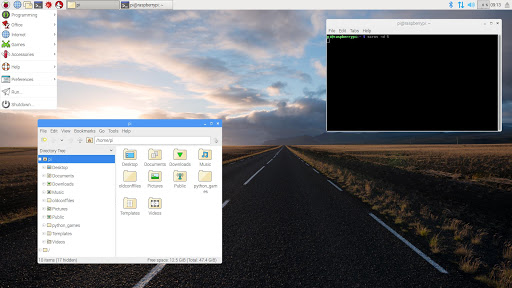
\includegraphics[width=0.5\textwidth]{img/Lab2_RBP_DP.jpg}
	\caption{Raspberry Pi 3B Desktop} 
	\label{BBD}
\end{figure}
%\imag 
\clearpage

\section{Connect to servo motor driver using i2c utility \& Control Servo motor using i2c utility \& Control Pan-tilt using c++ class}
\subsection{Setup}
In order to make the Raspberry Pi to control the I2C control board and the servo attach with it, following items is require.
\begin{itemize}
	\item Raspberry PI 3B
	\item SD card
	\item PCA9685
	\item Power Supply
	\item PTU
	\item Analog Discovery
\end{itemize}
\subsection{Procedure}
There are three processes to finish the goal.
\subsubsection{Enable the I2C Port in the Raspberry Pi}
The process to enable the I2C port in Raspberry Pi is following.
\begin{enumerate}[1)]
	\item Open Raspberry Pi command line.
	\item Run command \textbf{sudo rasp-config}
	\item Open \textbf{Interface} option and open \textbf{I2C Interface}
	\item reboot Raspberry Pi
\end{enumerate}
To testing the is the I2C working, type in command \textbf{gpio readall}, \textbf{ls /dev/*i2c*}, and \textbf{gpio i2cdetect} to show i2c device and check all the I2C slave in the bus.
\subsubsection{Adapt the Adafruit library to WiringPi environment}
Because the I2C board is manufactured by Adafruit, it provided a library to drive the PWM board. However, it only work on \textit{Arduino} platform. Therefore, it require some change in order to access the I2C device in the raspberry.
\\\\
After reading the library Adafruit provided, the structure of this program is very clear.
\begin{center}
	\textbf{uint8\_t read8(uint8\_t addr);}
	\textbf{void write8(uint8\_t addr, uint8\_t d);}
	\textbf{Adafruit\_PWMServoDriver();}
	\textbf{void begin(uint8\_t prescale = 0);}
\end{center}
All the function above is require to use the \textbf{wire.h} and \textbf{Arduino.h} and that need to be change to the WiringPi environment.
\begin{lstlisting}
Adafruit_PWMServoDriver::Adafruit_PWMServoDriver(){
	_i2caddr=0x70;	
}

void Adafruit_PWMServoDriver::begin(uint8_t prescale) {
	_i2c=wiringPiI2CSetup(_i2caddr);
	reset();
	if (prescale) {
		setExtClk(prescale);
	} else {
	// set a default frequency
		setPWMFreq(1000);
	}
	// set the default internal frequency
	setOscillatorFrequency(FREQUENCY_OSCILLATOR);
}

uint8_t Adafruit_PWMServoDriver::read8(uint8_t addr) {
	return wiringPiI2CReadReg8(_i2c,addr);
}

void Adafruit_PWMServoDriver::write8(uint8_t addr, uint8_t d) {
	wiringPiI2CWriteReg8 (_i2c, addr, d);

}
\end{lstlisting}
After apply those change and isolate the \textbf{wire.h} and \textbf{Arduino.h}, the program should be able to run in the Raspberry Pi environment.
\subsubsection{Testing circuit by attach servo and power supply}
To test the program follow process is required.
\begin{enumerate}[1)]
	\item Set up the power supply and set the output to \textbf{5V}
	\item Connect the power to the \textbf{V+} and \textbf{GND} port in PCA9685.
	\item Connect Raspberry Pi 3B 5v power to VCC and GND port in PCA9685.
	\item Connect Raspberry Pi 3B SCL, SDA to the same port in PCA9685.
	\item Set up Pull-Up resistor to SCL SDA and the VCC line.
	\item Connect Analog Discovery DIO0 and DIO1 to the SCL SDA port.
\end{enumerate}
After set up the hardware, use \textbf{gpio i2cdetect} to discovery the PCA9685 and the address of the PCA9685 is \textbf{0x40}.\\\\
To control the servo, program should have a \textit{Adafruit\_PWMServoDriver} object at the memory location \textbf{0x40}. Then, program will set up the frequency for the oscillator and update. In the end, the driver will set on the pwm frequency for each port.
\begin{lstlisting}
#define SERVO_FREQ 50
	int main(){
		Adafruit_PWMServoDriver pwm(0x40);
		pwm.begin();
		pwm.setOscillatorFrequency(27000000);
		pwm.setPWMFreq(SERVO_FREQ);
		int value=0;
		
		pwm.setPWM(0, 0, 350);
		pwm.setPWM(1, 0, 350);
		while(1){
			cin >> value;
			pwm.setPWM(0, 0, value);
		}
	}
\end{lstlisting}
This program will set up the pwm driver and apply pwm signal to the port. In the while loops, system will read the user input and use to adjust the servo.
\\\\
After testing the servo angle, controlling the Pan-tilt unit can be done by applying the correct pwm signal.
\subsection{Result}
By using \textbf{gpio i2cdetect}, the address for the servo driver is 0x40.
\begin{figure}[hb]
	\centering
	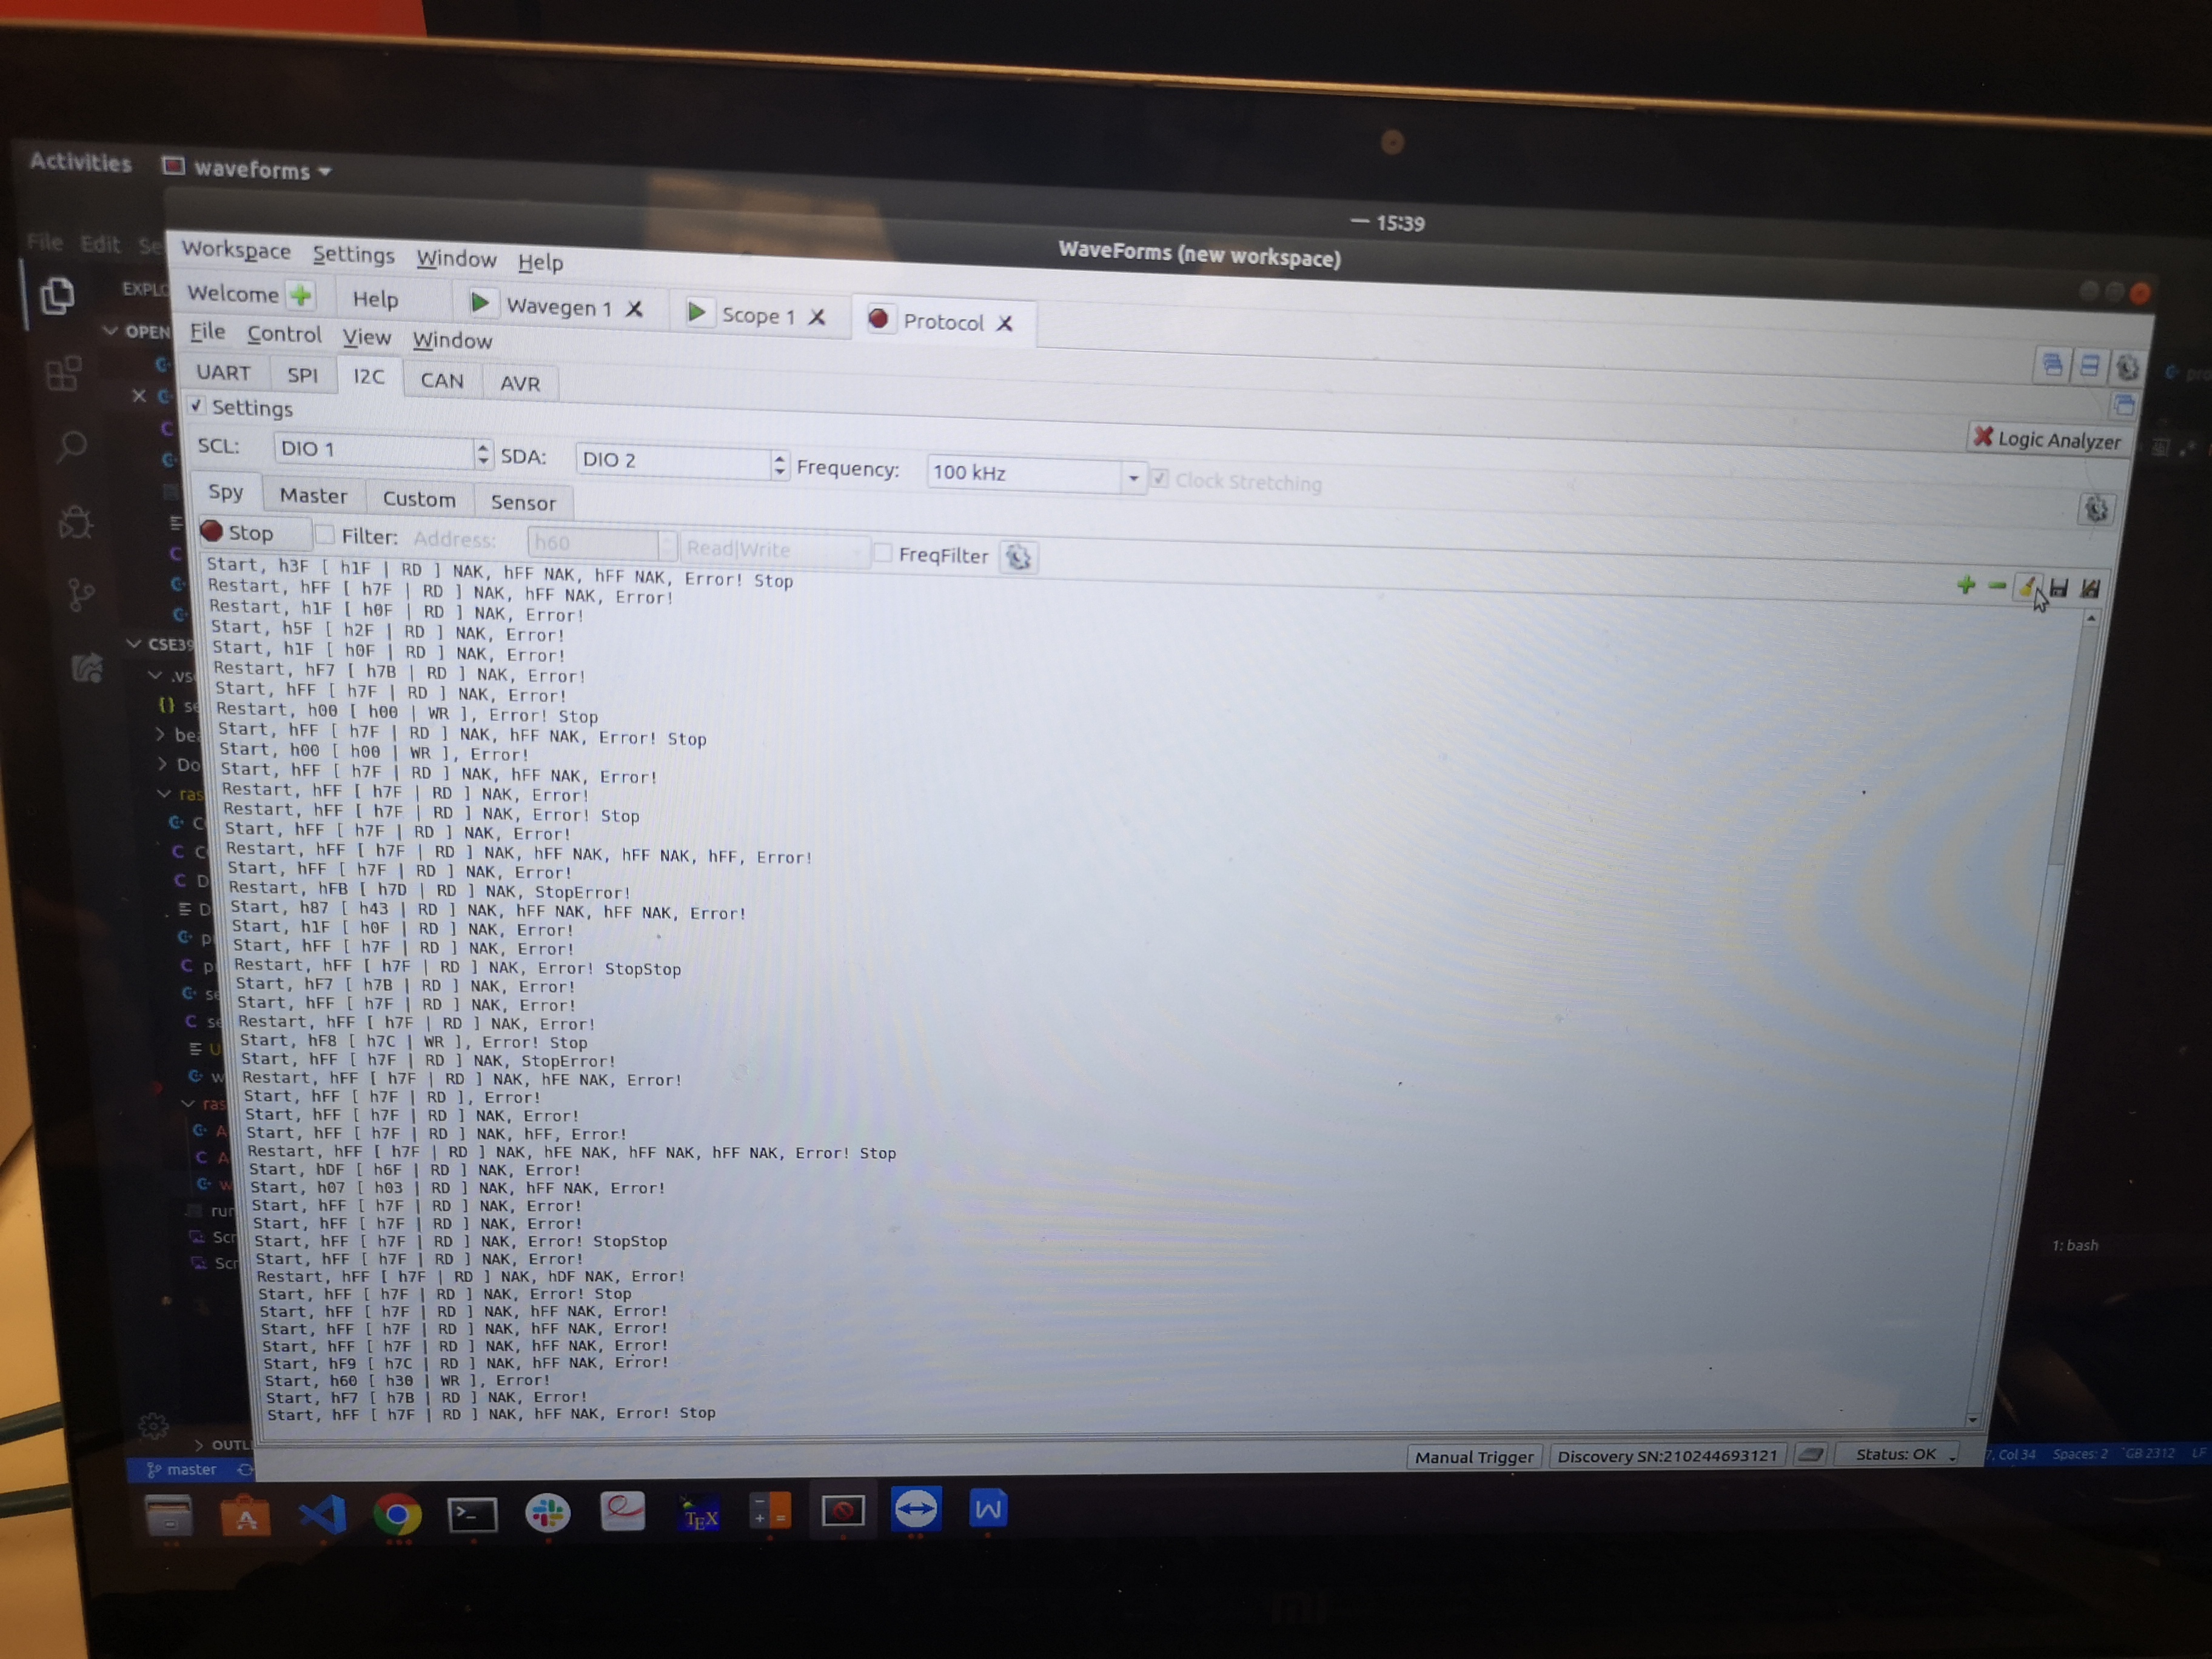
\includegraphics[width=0.5\textwidth]{img/Lab03_04.jpg}
	\caption{I2C Reading From Analog Discovery} 
	\label{BBD}
\end{figure}
By using the angle testing program, the pwm range is from 250 to 420.
\begin{figure}[hb]
	\centering
	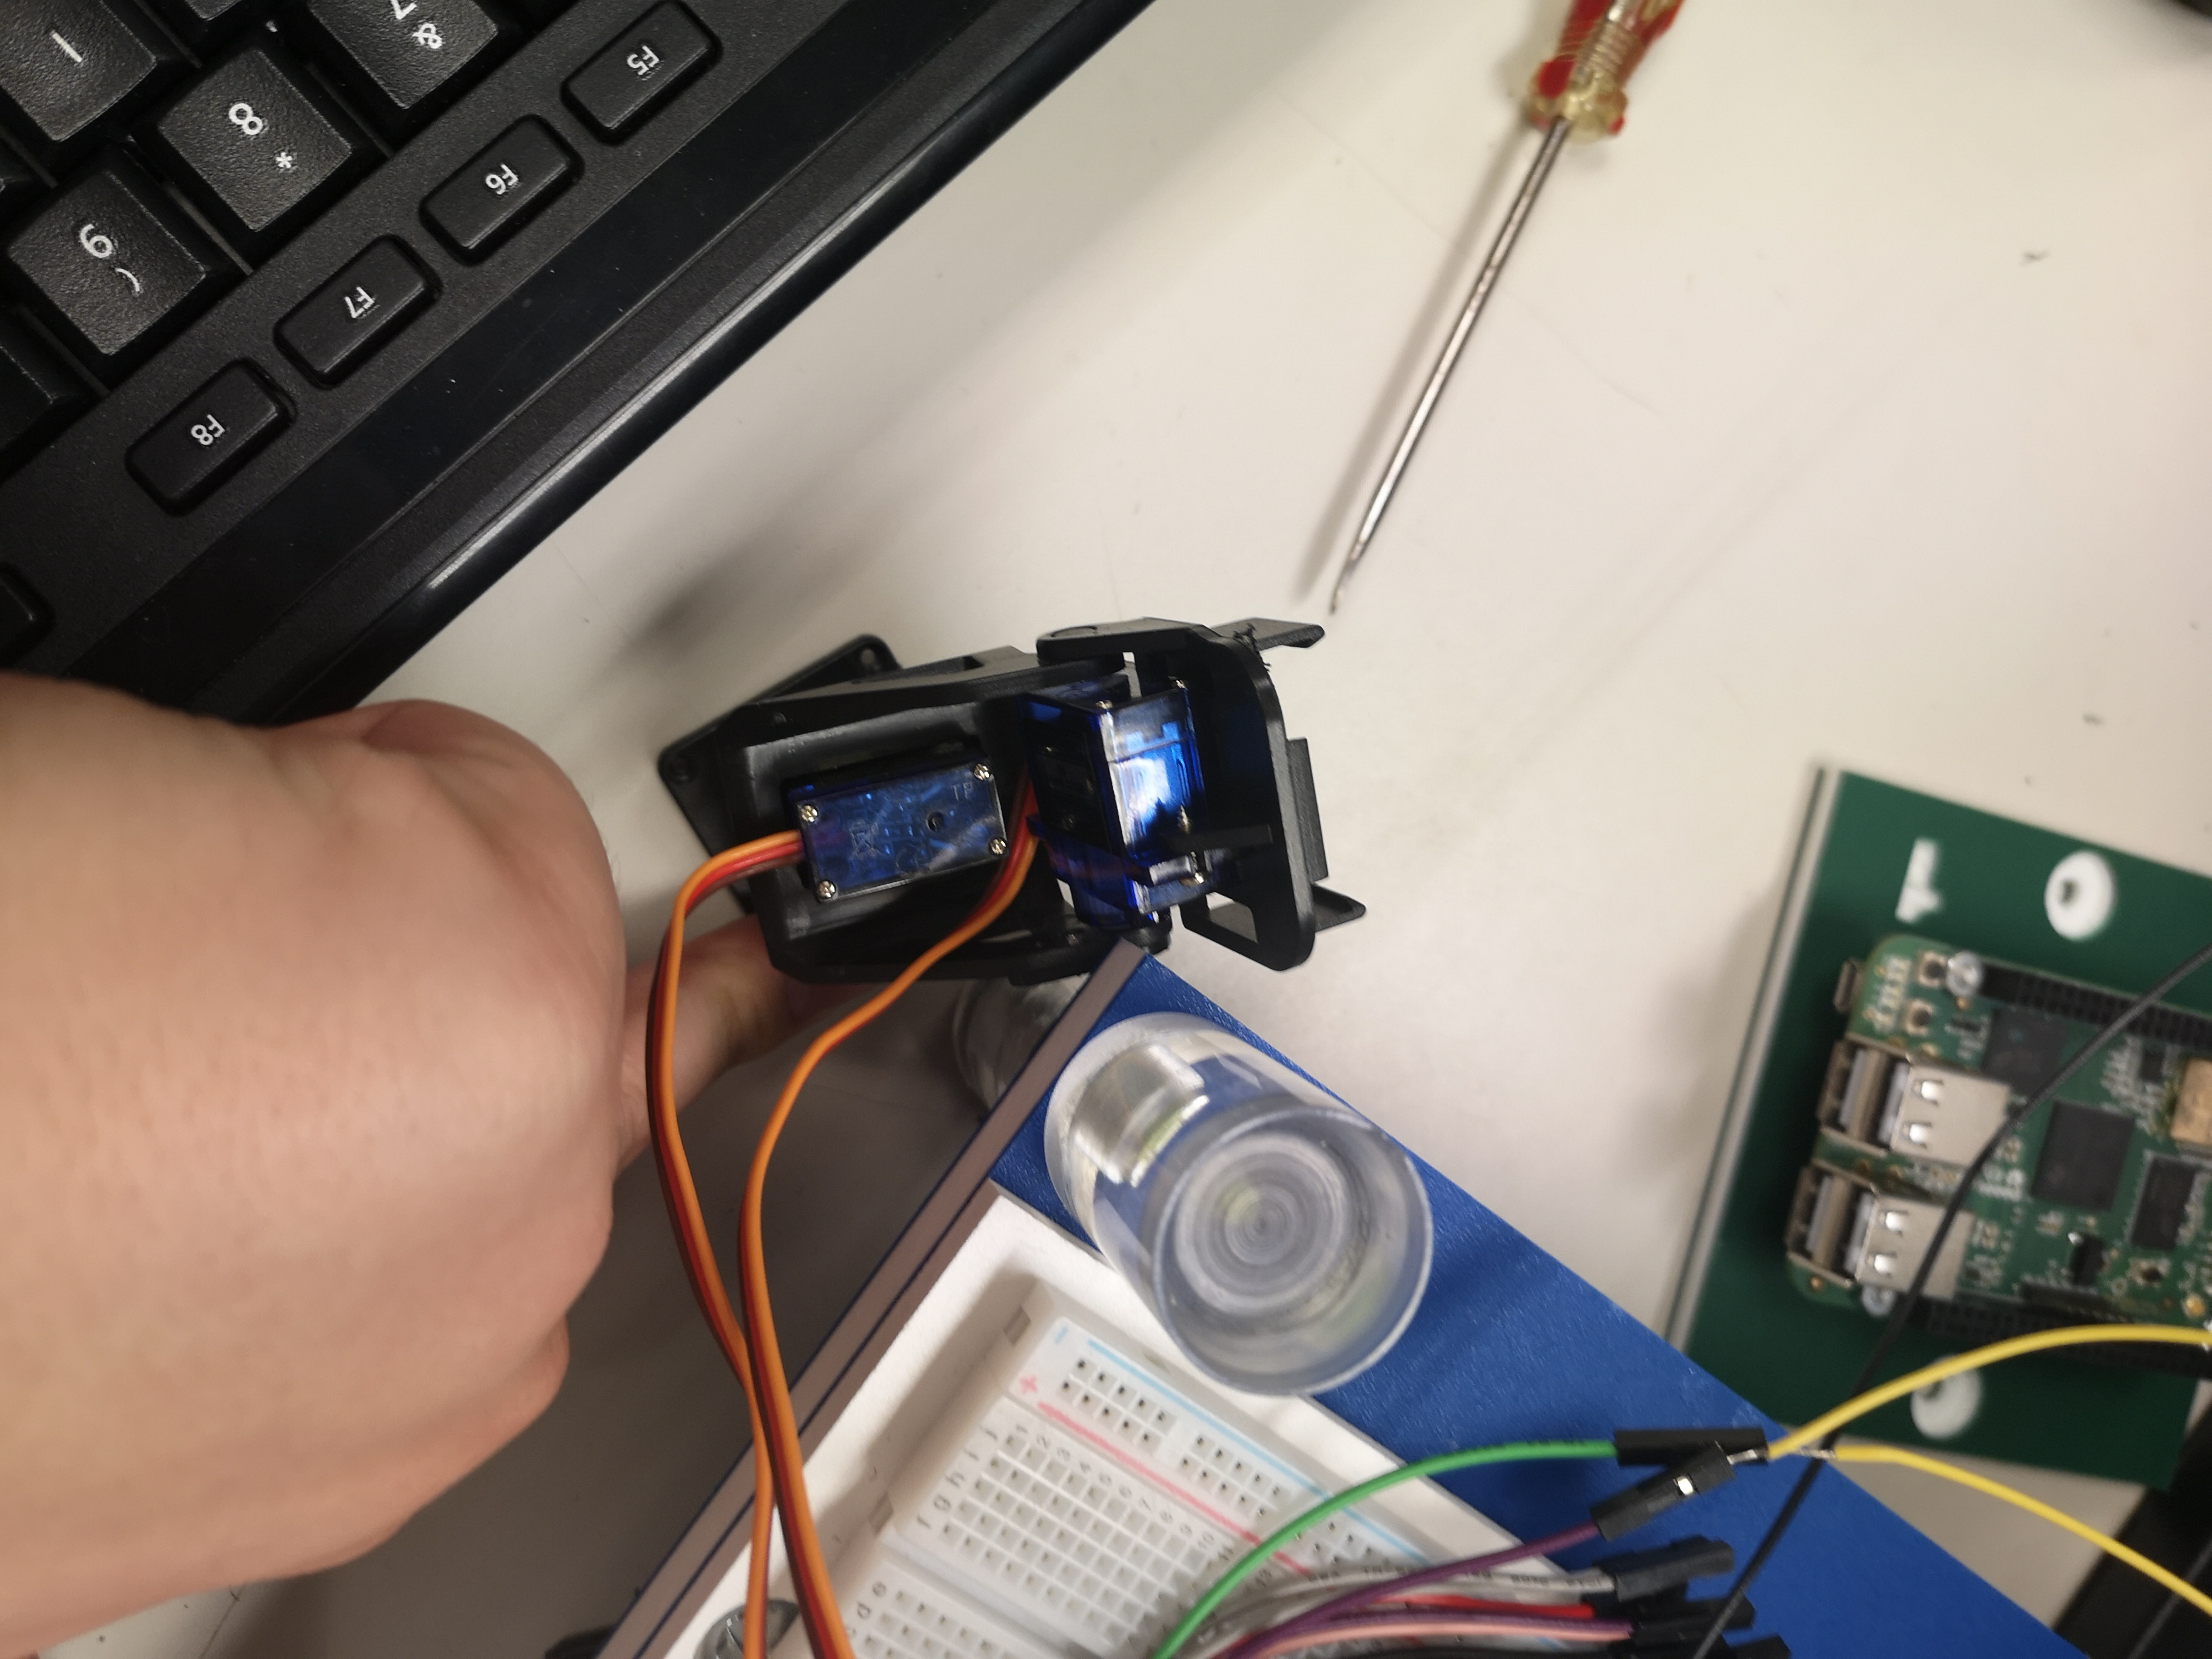
\includegraphics[width=0.5\textwidth]{img/Lab03_06.jpg}
	\caption{Pan-tilt Unit} 
	\label{BBD}
\end{figure}
After using apply all the program into the system, the pan-tilt will point to the target input into the system.
\begin{figure}[hb]
	\centering
	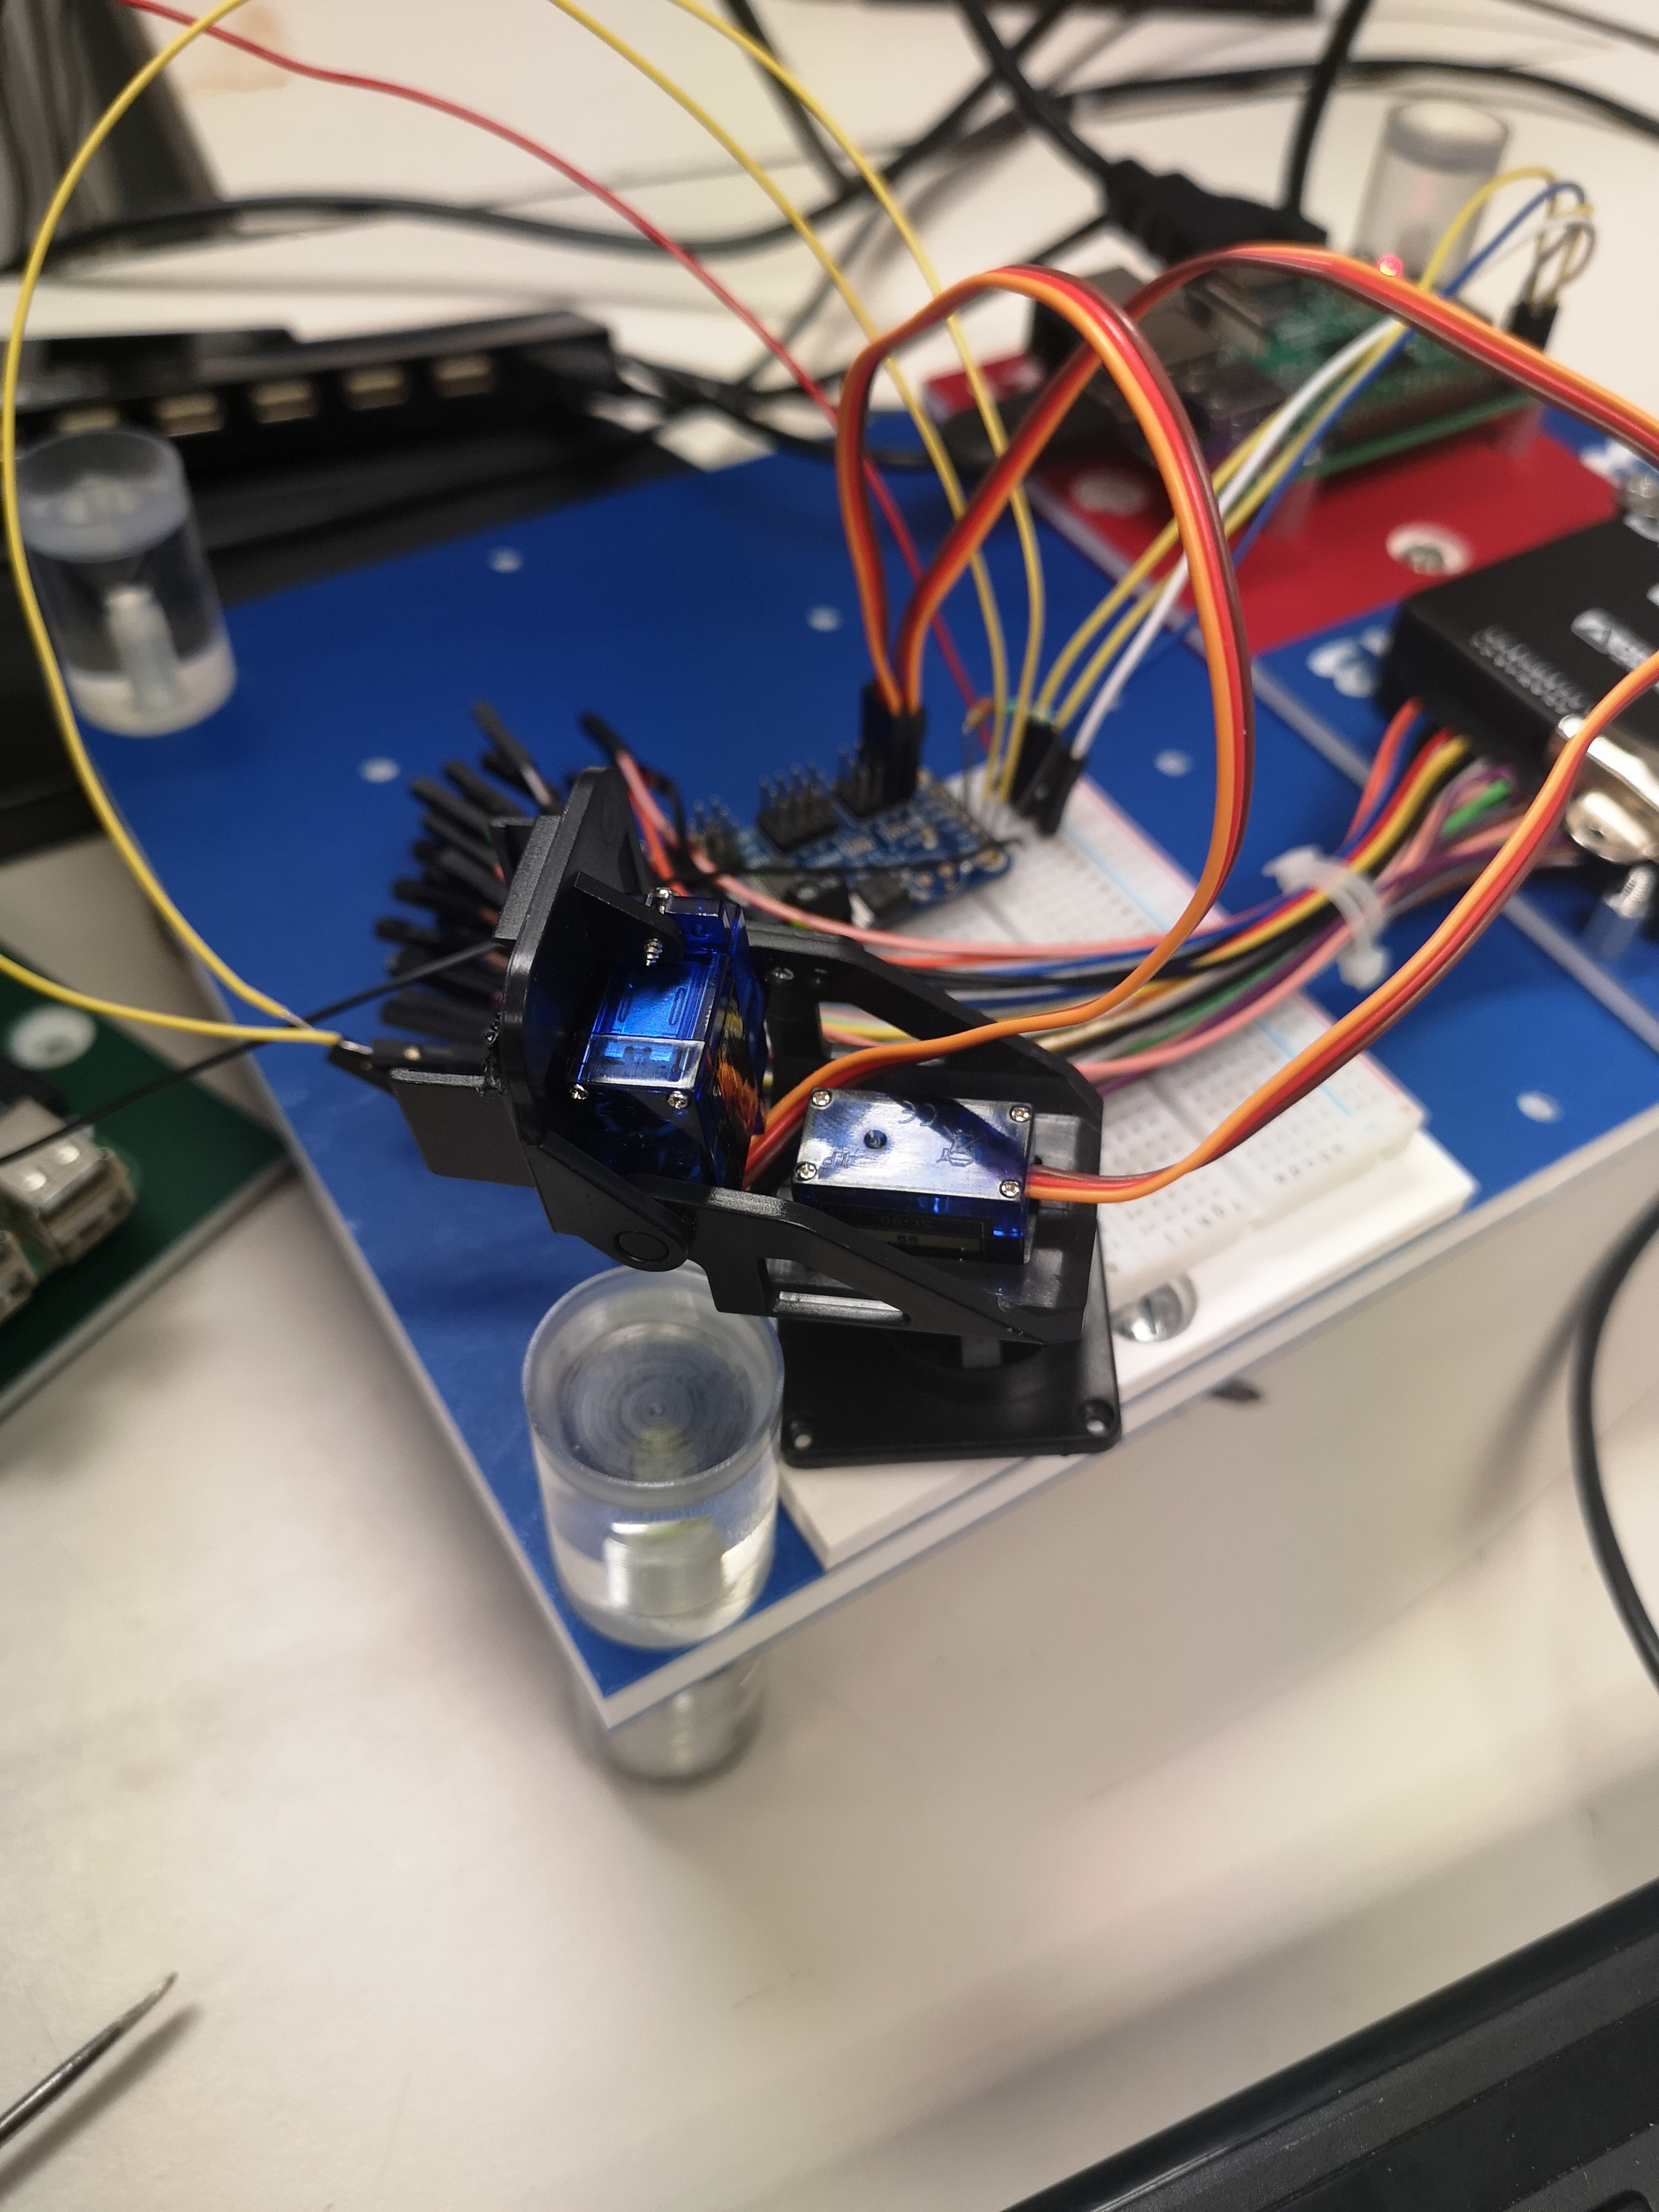
\includegraphics[width=0.5\textwidth]{img/Lab03_01.jpg}
	\caption{Pan-tilt Unit with Pointing} 
	\label{BBD}
\end{figure}
\clearpage





\section{Connect your phone to RPi using Bluetooth}
\subsection{Setup}
In order to make the Raspberry Pi to control the Bluetooth, following items is require.
\begin{itemize}
	\item Raspberry PI 3B
	\item SD card
	\item Analog Discovery
\end{itemize}
\subsection{Procedure}
The process to enable the Bluetooth port in Raspberry Pi is following.
\begin{enumerate}[1)]
	\item Open Raspberry Pi command line.
	\item Run command \textbf{sudo rasp-config}
	\item Open \textbf{Interface} option and open \textbf{Bluetooth Interface}
	\item reboot Raspberry Pi
	\item Run command \textbf{sudo bluetoothctl} to start the bluetoothctl
	\item Run command in bluetoothctl \textbf{power on} to enable the power setting
	\item Run command in bluetoothctl \textbf{agent on} to start the agent
	\item Run command in bluetoothctl \textbf{discoverable on} to allow disable
	\item Run command in bluetoothctl \textbf{default-agent} to use the default agent
	\item Use phone to find the raspberry-pi bluetooth device.
	\item Confirm the pair request and trust the device.
	\item Run following command in command line
	\begin{center}
		hciconfig hci0 piscan
	\end{center}
	\begin{center}
		sdptool add SP
	\end{center}
	\item Run command \textbf{sudo apt-get install libbluetooth-dev}
\end{enumerate}
The following program is provide by TA. By running this program, phone which connect to the raspberry will receive a message from the Raspberry Pi.
\begin{lstlisting}
#include <stdio.h>
#include <unistd.h>
#include <sys/socket.h>
#include "bluetooth.h"
#include "rfcomm.h"

using namespace std;
int main(int argc, char **argv)
{
	struct sockaddr_rc loc_addr = { 0 }, rem_addr = { 0 };
	char buf[1024] = { 0 };
	int s, client, bytes_read;
	socklen_t opt = sizeof(rem_addr);
	
	// allocate socket
	s = socket(AF_BLUETOOTH, SOCK_STREAM, BTPROTO_RFCOMM);
	
	// bind socket to port 1 of the first available 
	// local bluetooth adapter
	loc_addr.rc_family = AF_BLUETOOTH;
	//loc_addr.rc_bdaddr = *BDADDR_ANY;
	loc_addr.rc_channel = (uint8_t) 1;
	bind(s, (struct sockaddr *)&loc_addr, sizeof(loc_addr));
	
	// put socket into listening mode
	listen(s, 1);
	
	// accept one connection
	client = accept(s, (struct sockaddr *)&rem_addr, &opt);
	
	ba2str( &rem_addr.rc_bdaddr, buf );
	fprintf(stderr, "accepted connection from %s\n", buf);
	memset(buf, 0, sizeof(buf));
	
	// read data from the client
	bytes_read = read(client, buf, sizeof(buf));
	if( bytes_read > 0 ) {
		printf("received [%s]\n", buf);
	}
	
	// close connection
	close(client);
	close(s);
	return 0;
}
\end{lstlisting}
\clearpage
\subsection{Result}
After follow the procedure above, the phone successfully connect to the Raspberry Pi and receive the default message.
\begin{figure}[hb]
	\centering
	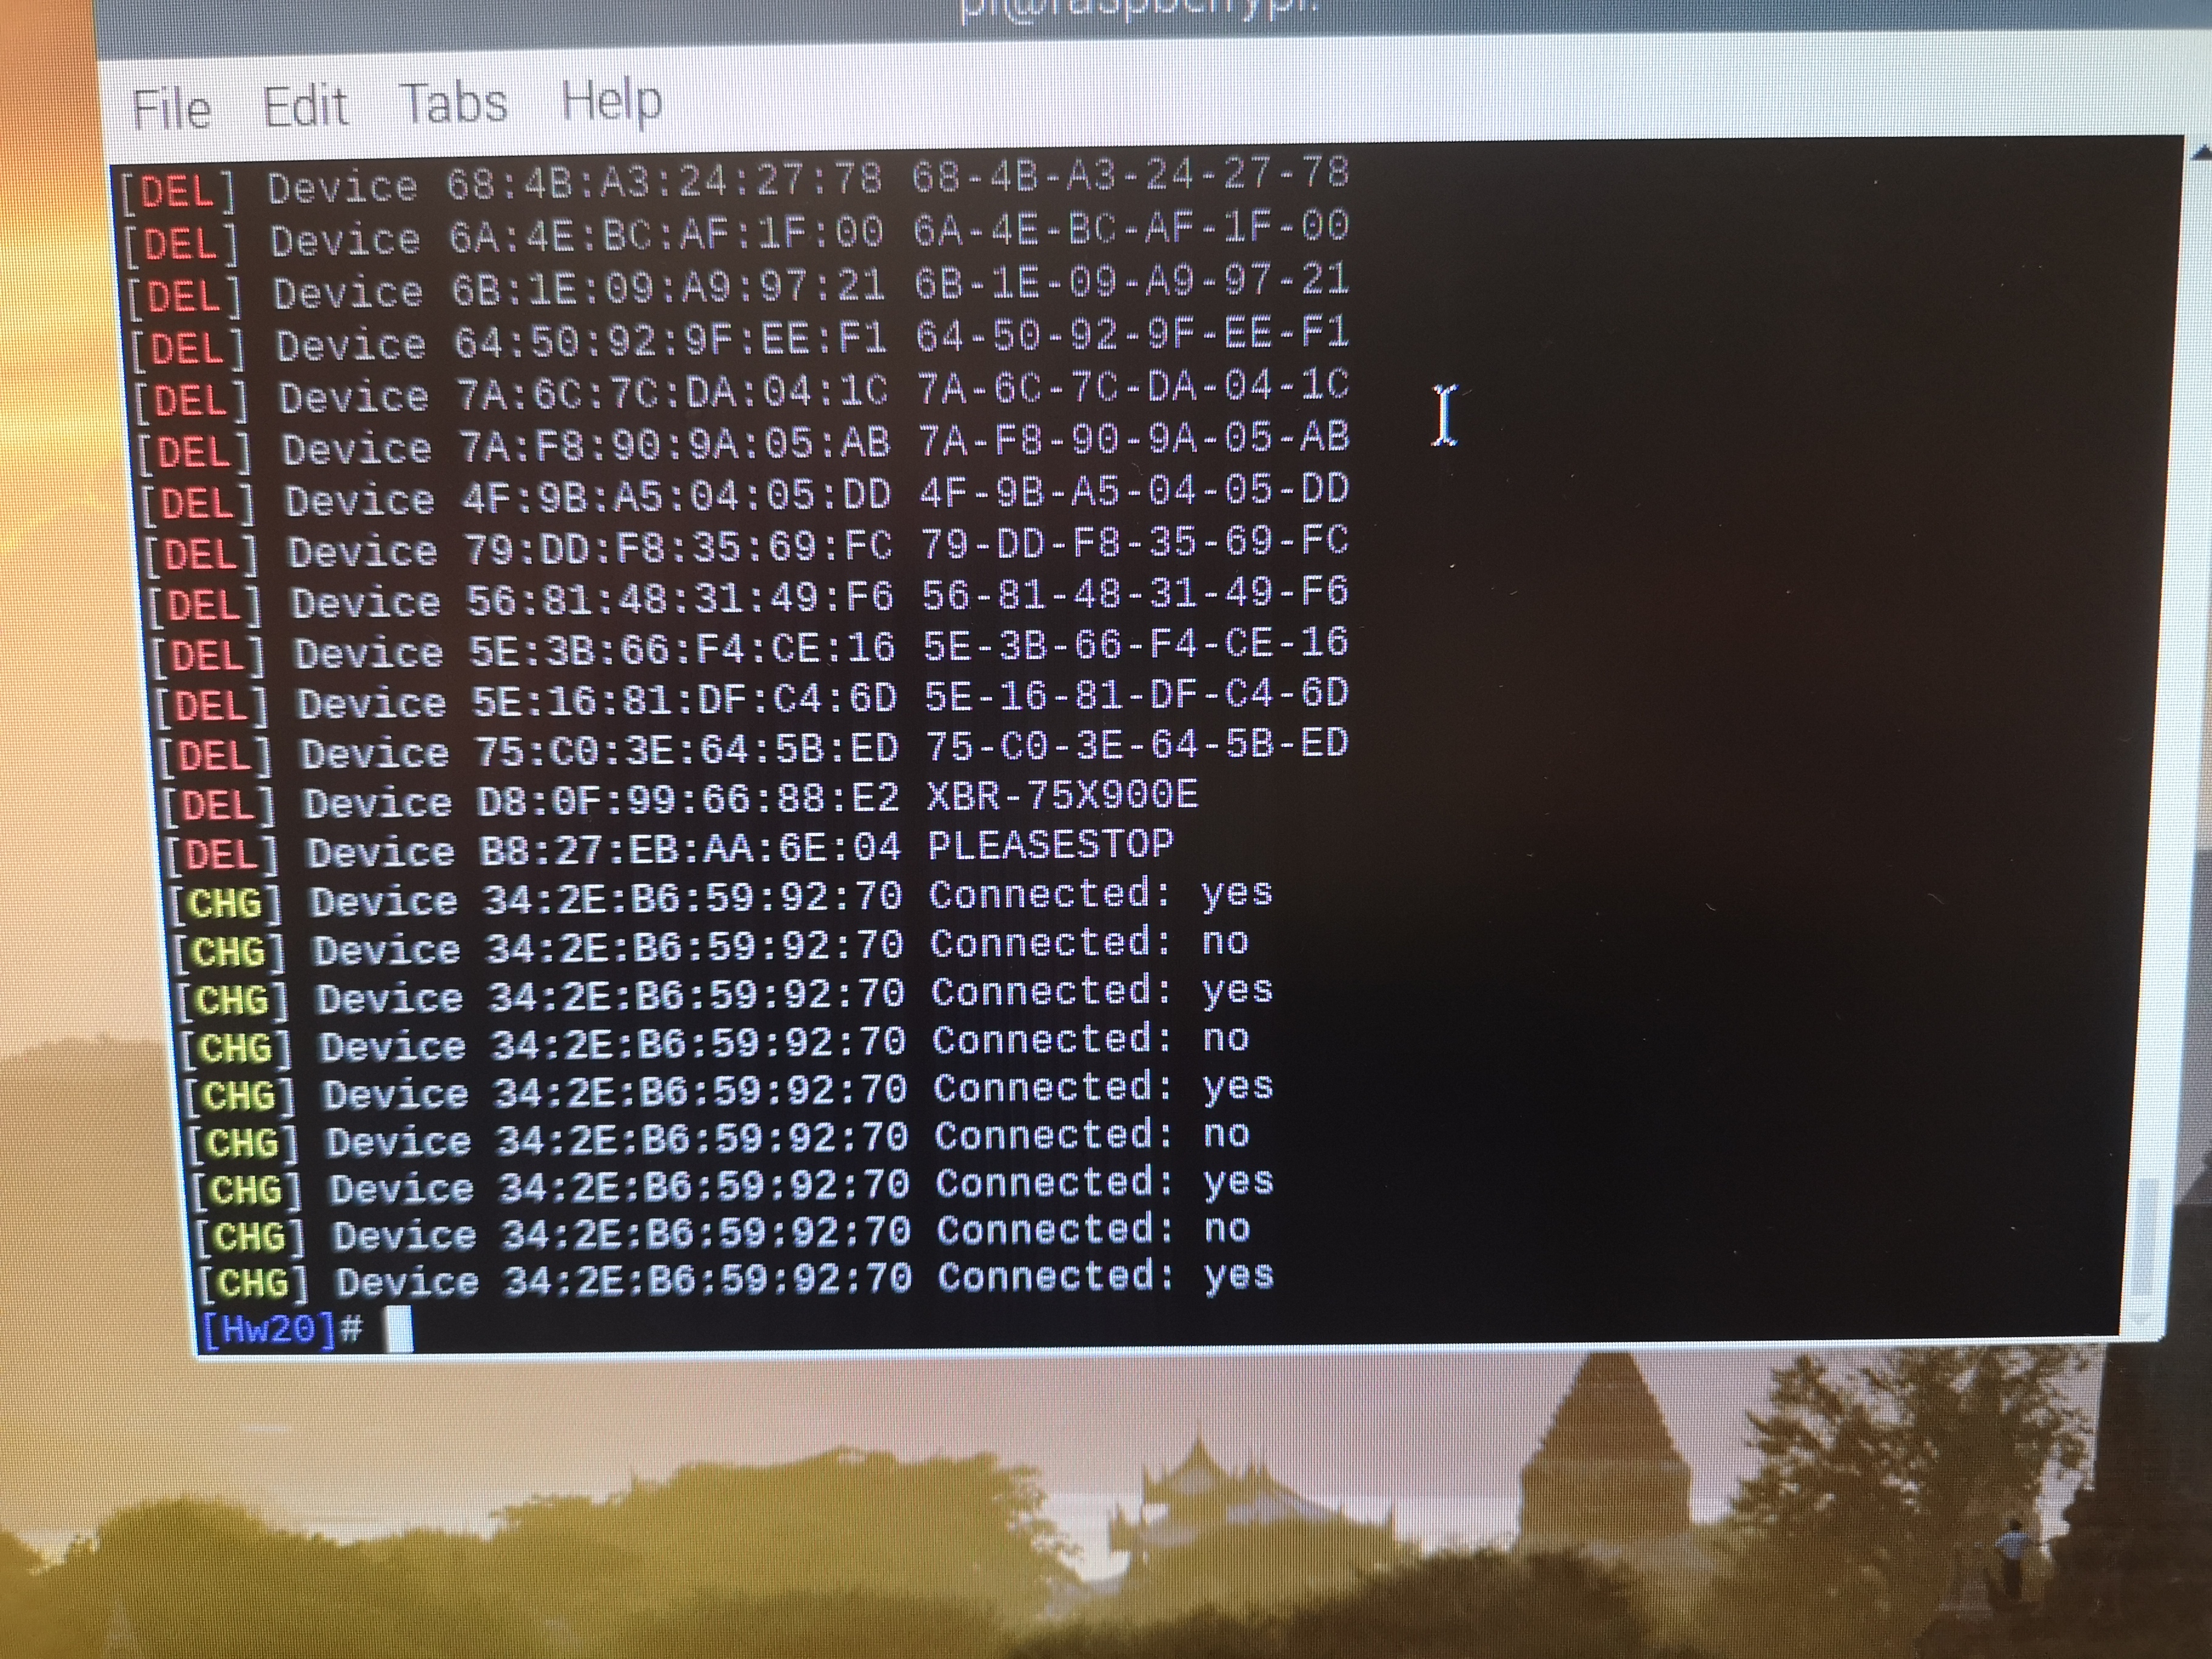
\includegraphics[width=0.5\textwidth]{img/Lab03_12.jpg}
	\caption{Bluetooth Connection} 
	\label{BBD}
\end{figure}
\clearpage


\section{Send data to RPi using a BT class and app \& Control PTU using your phone}
\subsection{Setup}
In order to make the Raspberry Pi to control the I2C control board and the servo attach with it by bluetooth, following items is require.
\begin{itemize}
	\item Raspberry PI 3B
	\item SD card
	\item PCA9685
	\item Power Supply
	\item Analog Discovery
	\item PTU
\end{itemize}
\subsection{Procedure}
The process of allow connection between the pwm servo and the bluetooth take three major steps.
\subsubsection{Program the bluetooth class}
By reading the program, the structure can be discovery. The way program and bluetooth communication by file describer. It indicate it is possible to send the data out by use the \textbf{write} function call.
\begin{lstlisting}
    rfcomm_server& operator<<(std::string s){
		write(client,s.c_str(),s.size());
		write(client,"\n",1);
		return *this;
	}
	rfcomm_server& operator>>(std::string* s){
		char buf[1024] = { 0 };
		int bytes_read=-1;
		while (bytes_read==-1){
			memset(buf, 0, sizeof(buf));
			bytes_read= read(client, buf, sizeof(buf));
		}
		s->append(buf);
		return *this;
	}
\end{lstlisting}
\subsubsection{Connect the bluetooth and send out a message}
By using the previous created class, a small program can be created to test the class and the ability to transmit message. Statement \textbf{rfcomm\_server rout} and \textbf{rout<< "good news"}.
\subsubsection{Connect the bluetooth and pwm servo}
By using the previous created classes, it will be easy to create a program to use bluetooth to control the servo.
The program contain two parts. The first part is to setup the I2C connection and the bluetooth connection. The second part is read the message that came from the bluetooth and use this value to update pwm signal.
\subsection{Result}
When testing the bluetooth, the phone will receive a \textbf{good news} message from the raspberry pi.
\begin{figure}[hb]
	\centering
	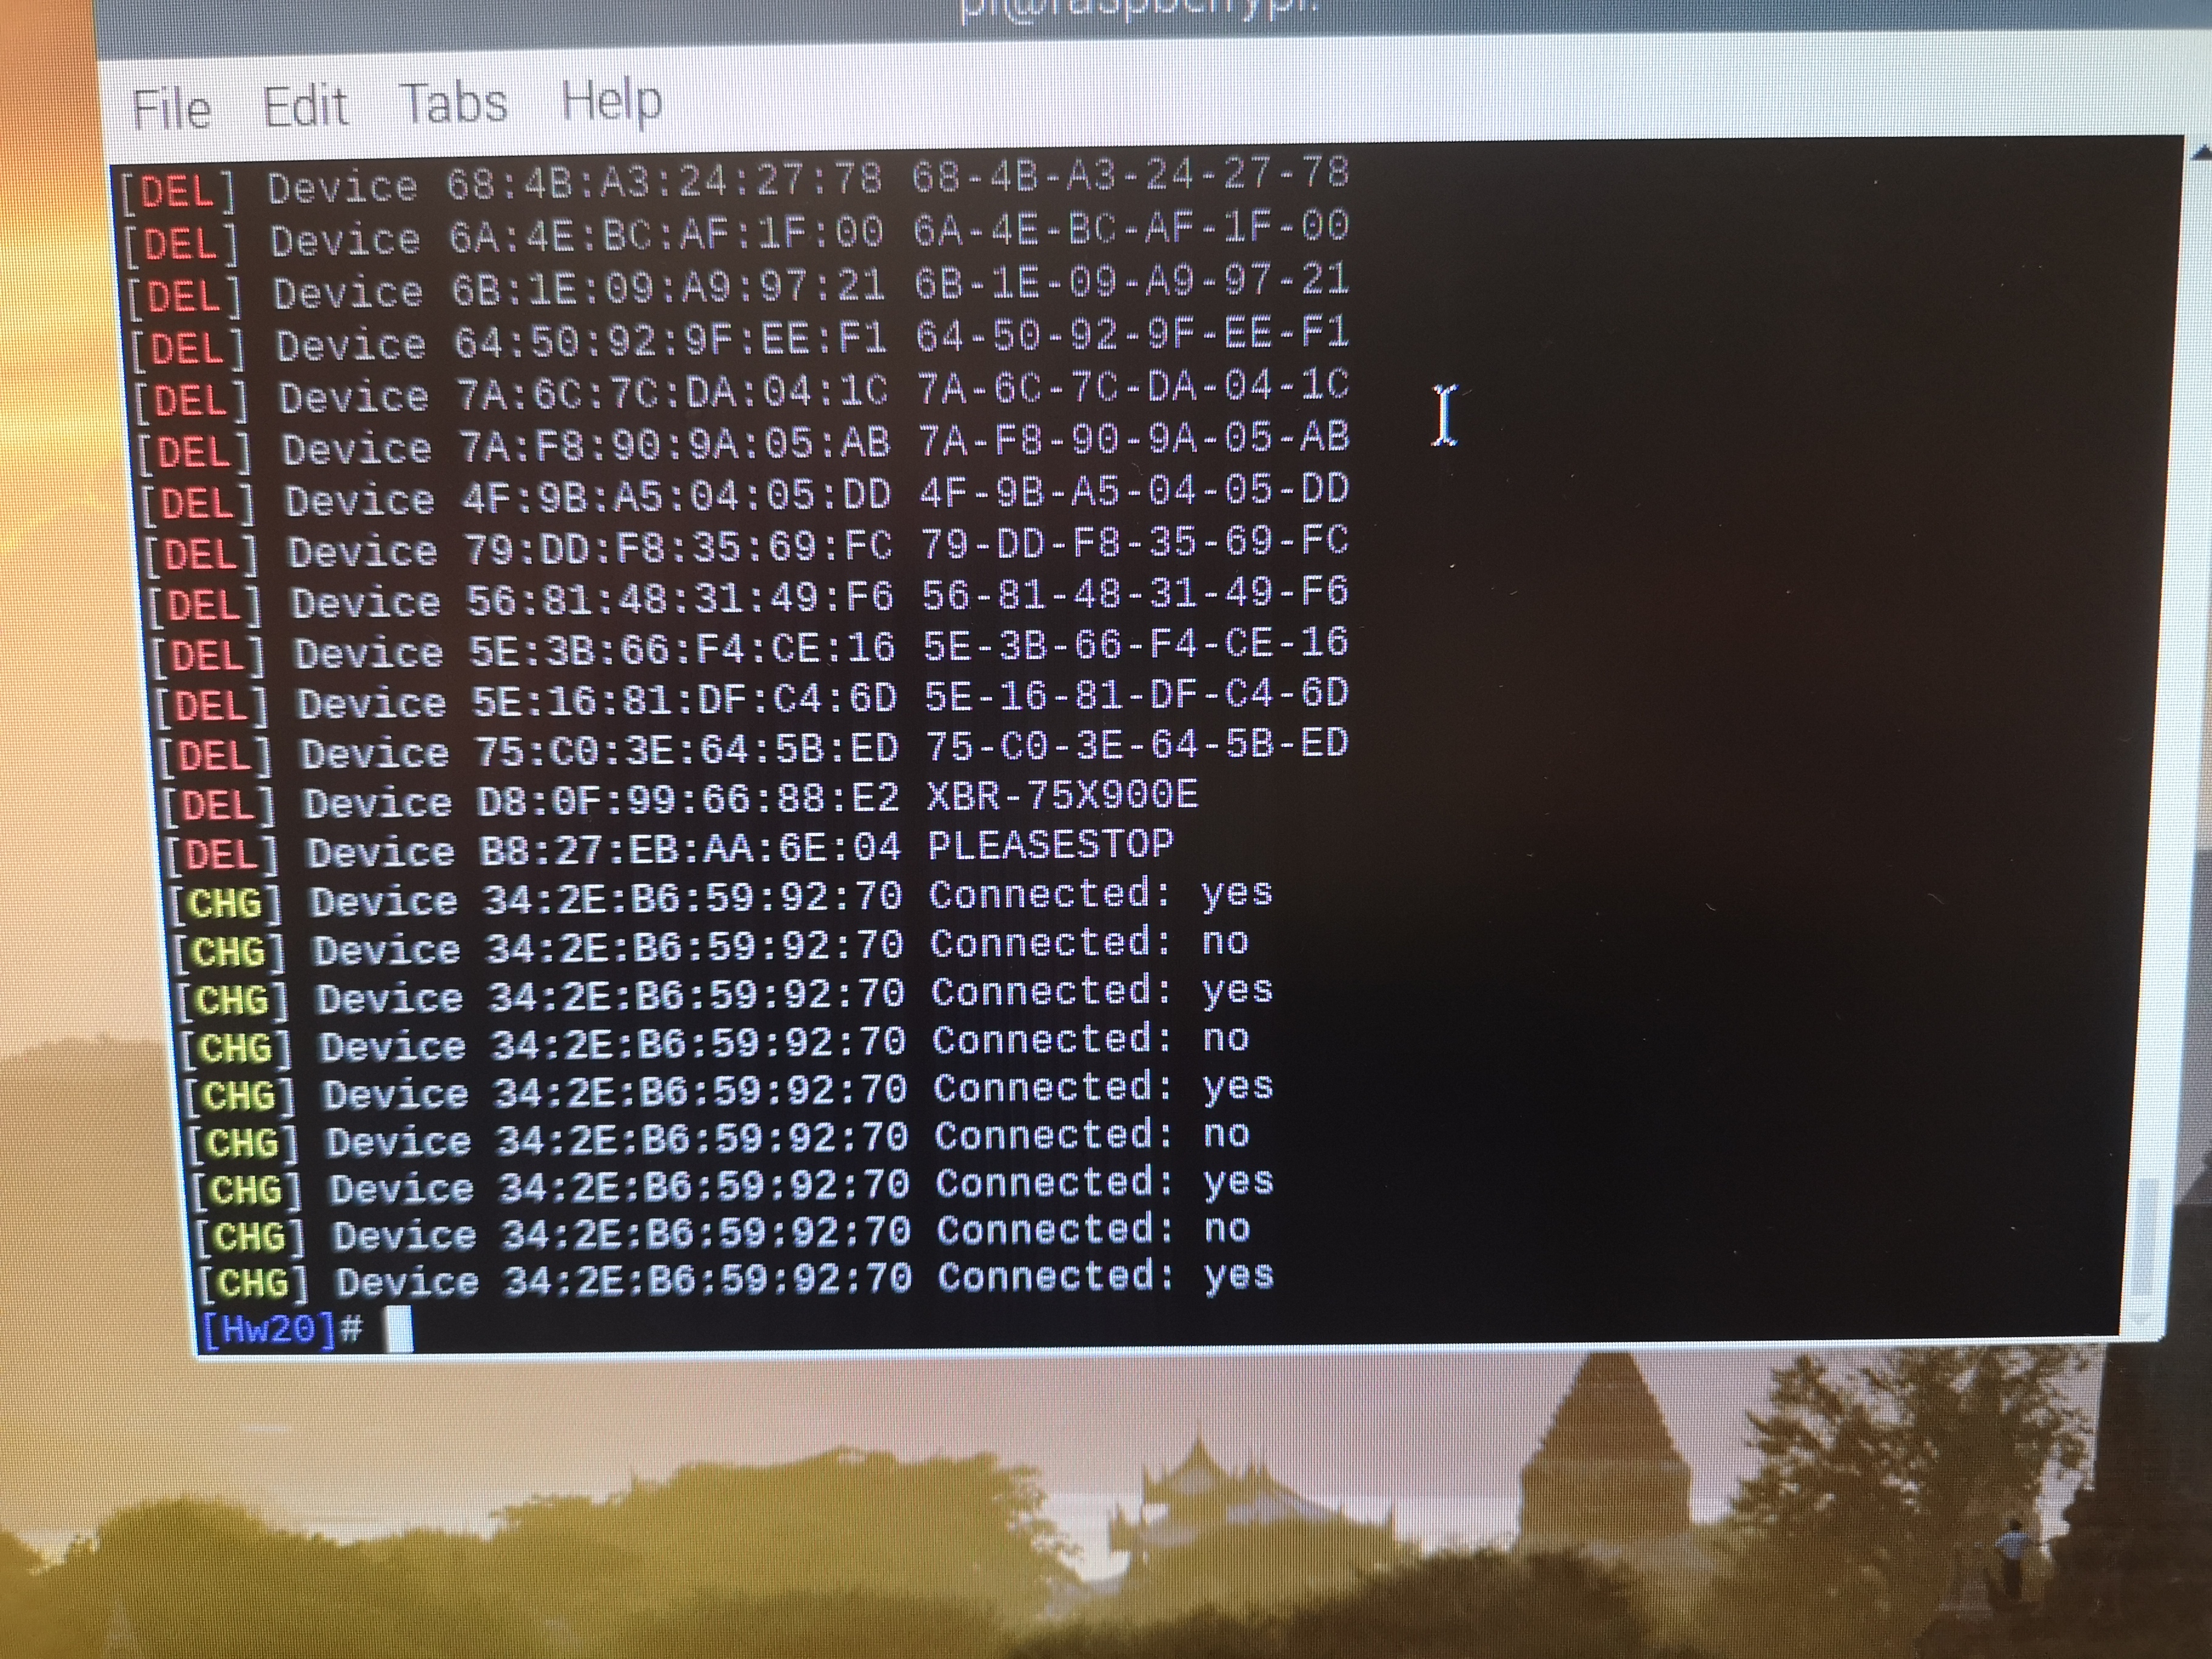
\includegraphics[width=0.5\textwidth]{img/Lab03_12.jpg}
	\caption{Bluetooth Connection} 
	\label{BBD}
\end{figure}
When using the bluetooth to control the servo, the servo will move to pre-programmed location base on the command phone send out. 
\begin{figure}[hb]
	\centering
	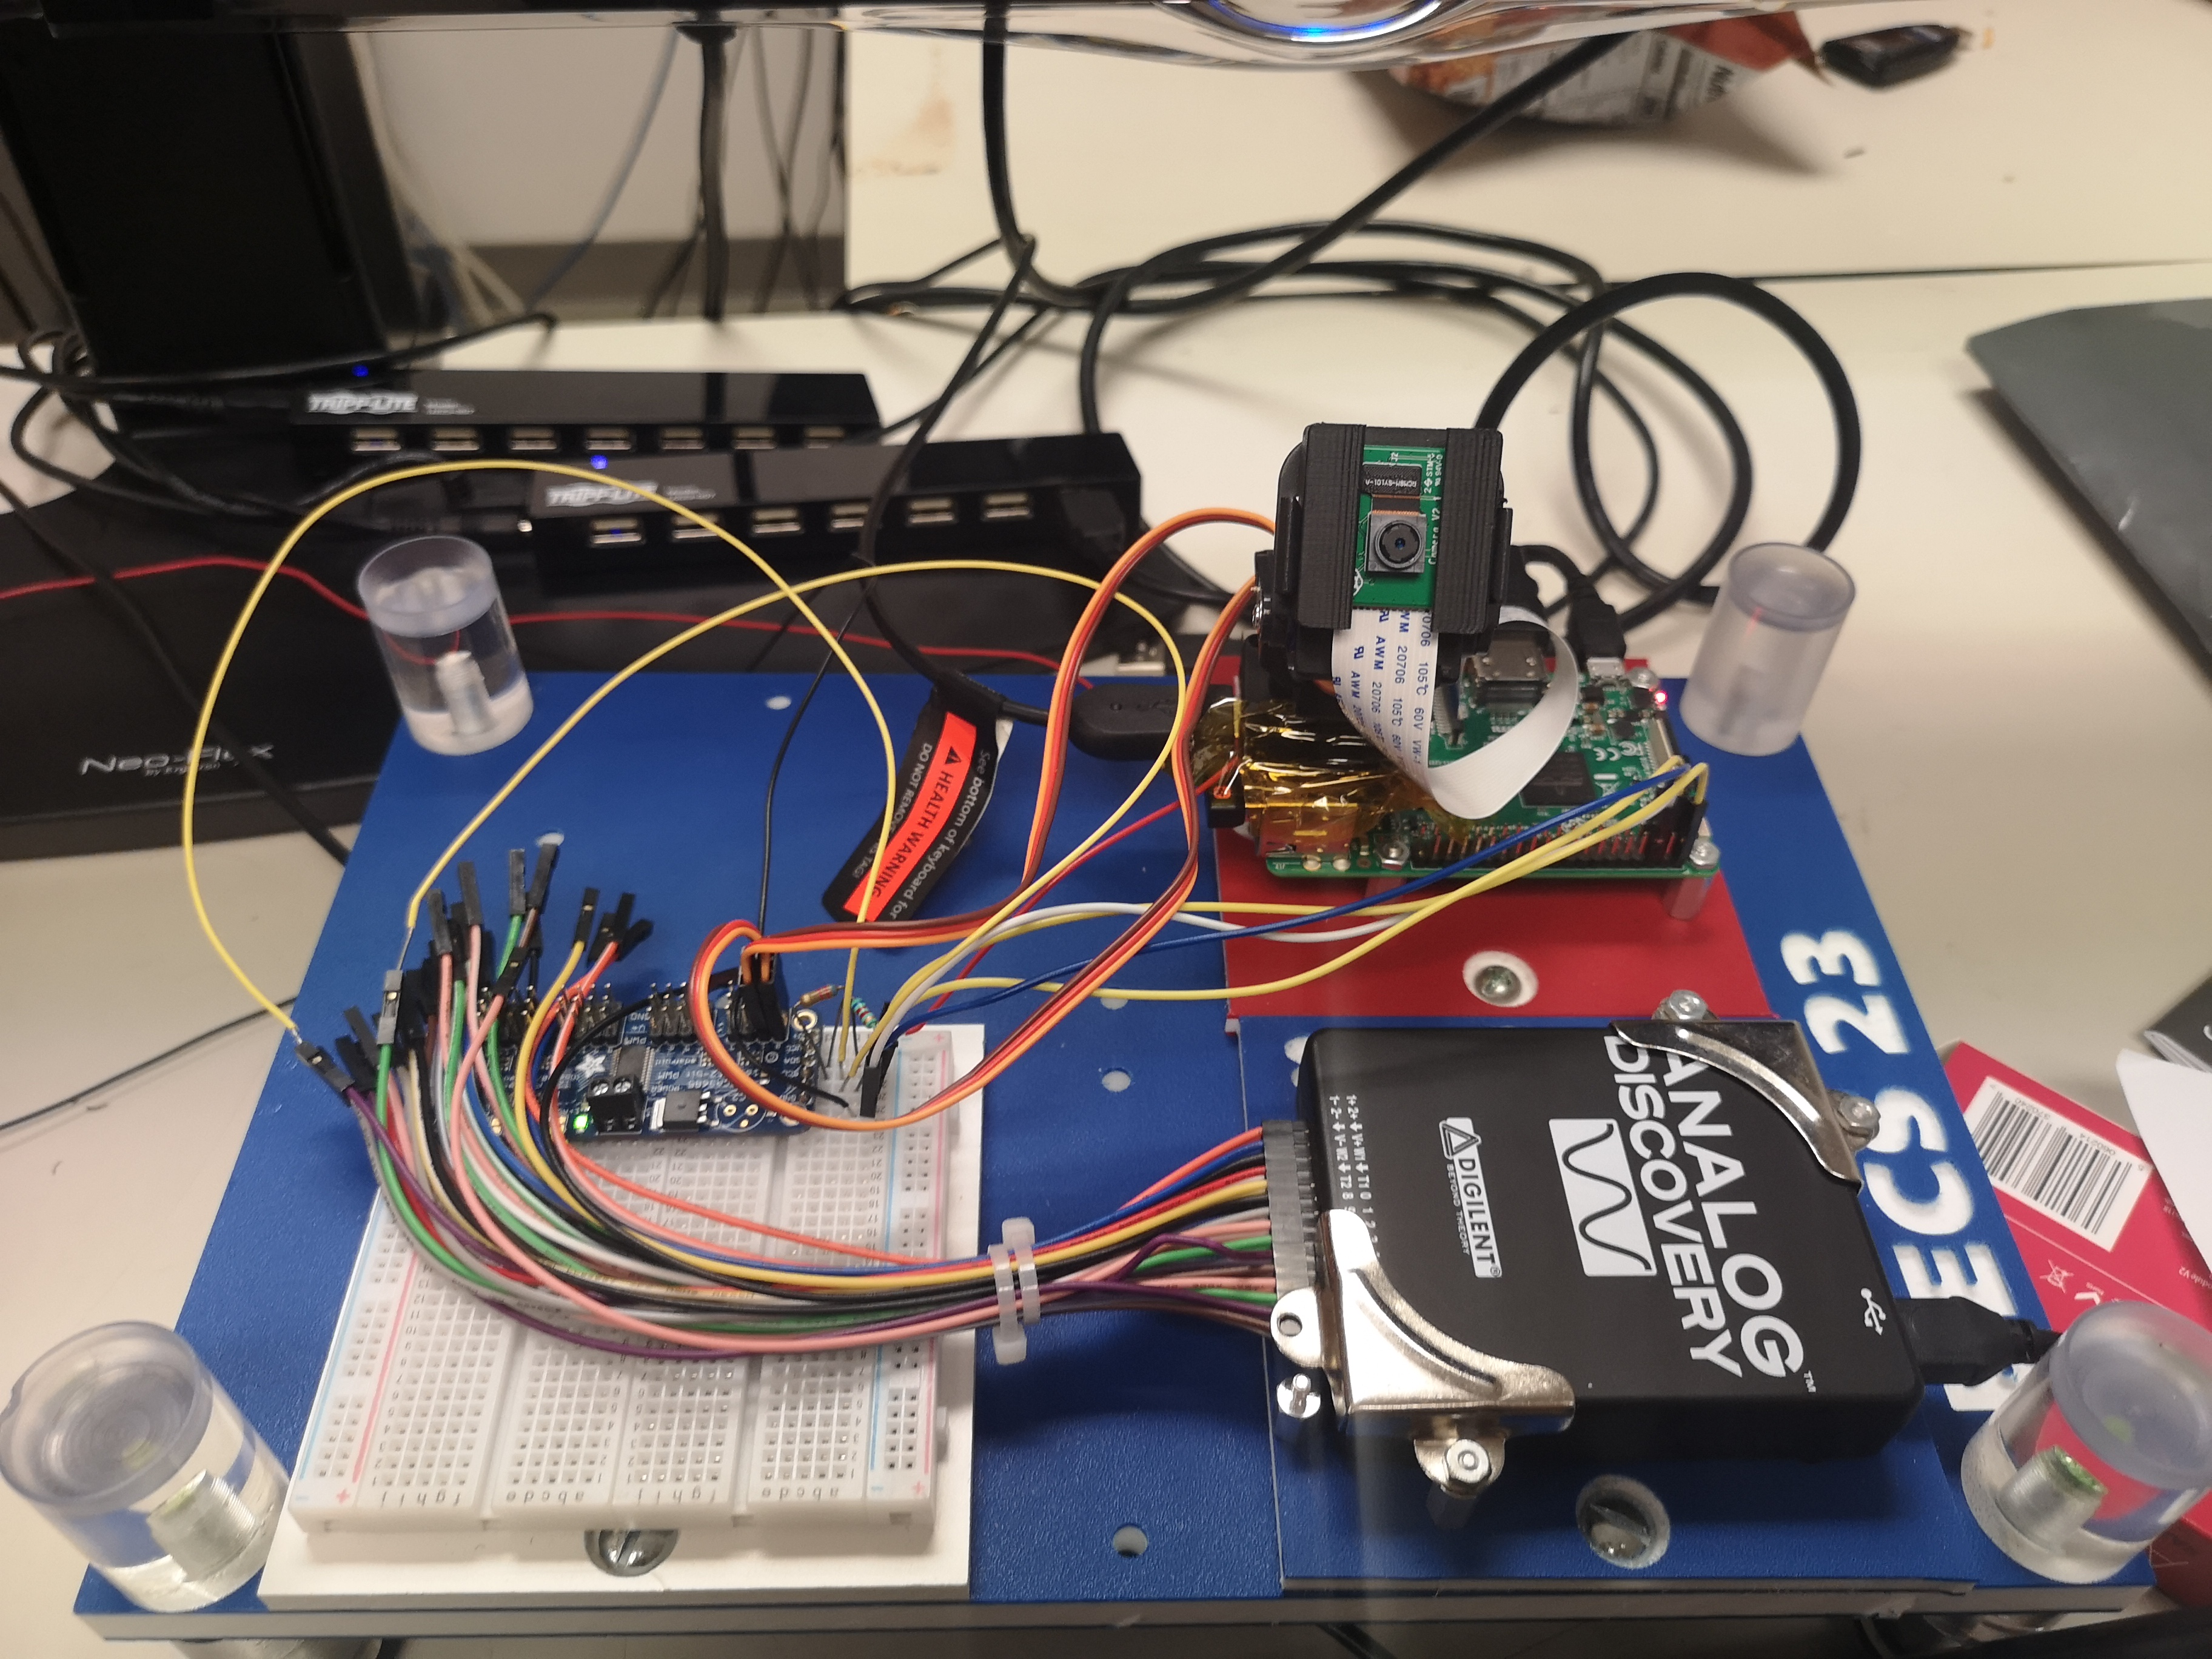
\includegraphics[width=0.5\textwidth]{img/Lab03_10.jpg}
	\caption{WorkBranch Setup} 
	\label{BBD}
\end{figure}
\clearpage

\section{Get image using camera and raspistill}
\subsection{Setup}
In order to make the Raspberry Pi to get image using camera and raspistill, following items is require.
\begin{itemize}
	\item Raspberry PI 3B
	\item SD card
	\item Raspberry Camera
\end{itemize}
\subsection{Procedure}
Install the camera of the Raspberry Pi require the Raspberry Pi to power off during the installation of the camera. Becasuse the sensor in the camera is very sensitive, installing the camera with power will cause a power pulse on the camera sensor and destroy the sensor in the camera. After start the Raspberry with the camera. Following steps is required to start the camera.
\begin{enumerate}
	\item Run following command in the command line \textbf{sudo rasp-config}
	\item In the config pag, open the \textbf{interface} page and turn on the \textbf{camera} option.
	\item After exist the config page, reboot the system.
	\item After finish reboot, run command in the command line \textbf{raspistill -o text.jpg}
\end{enumerate}
\subsection{Result}
After run thought all command above, a image will be in the home directory call "text.jpg".
\begin{figure}[hb]
	\centering
	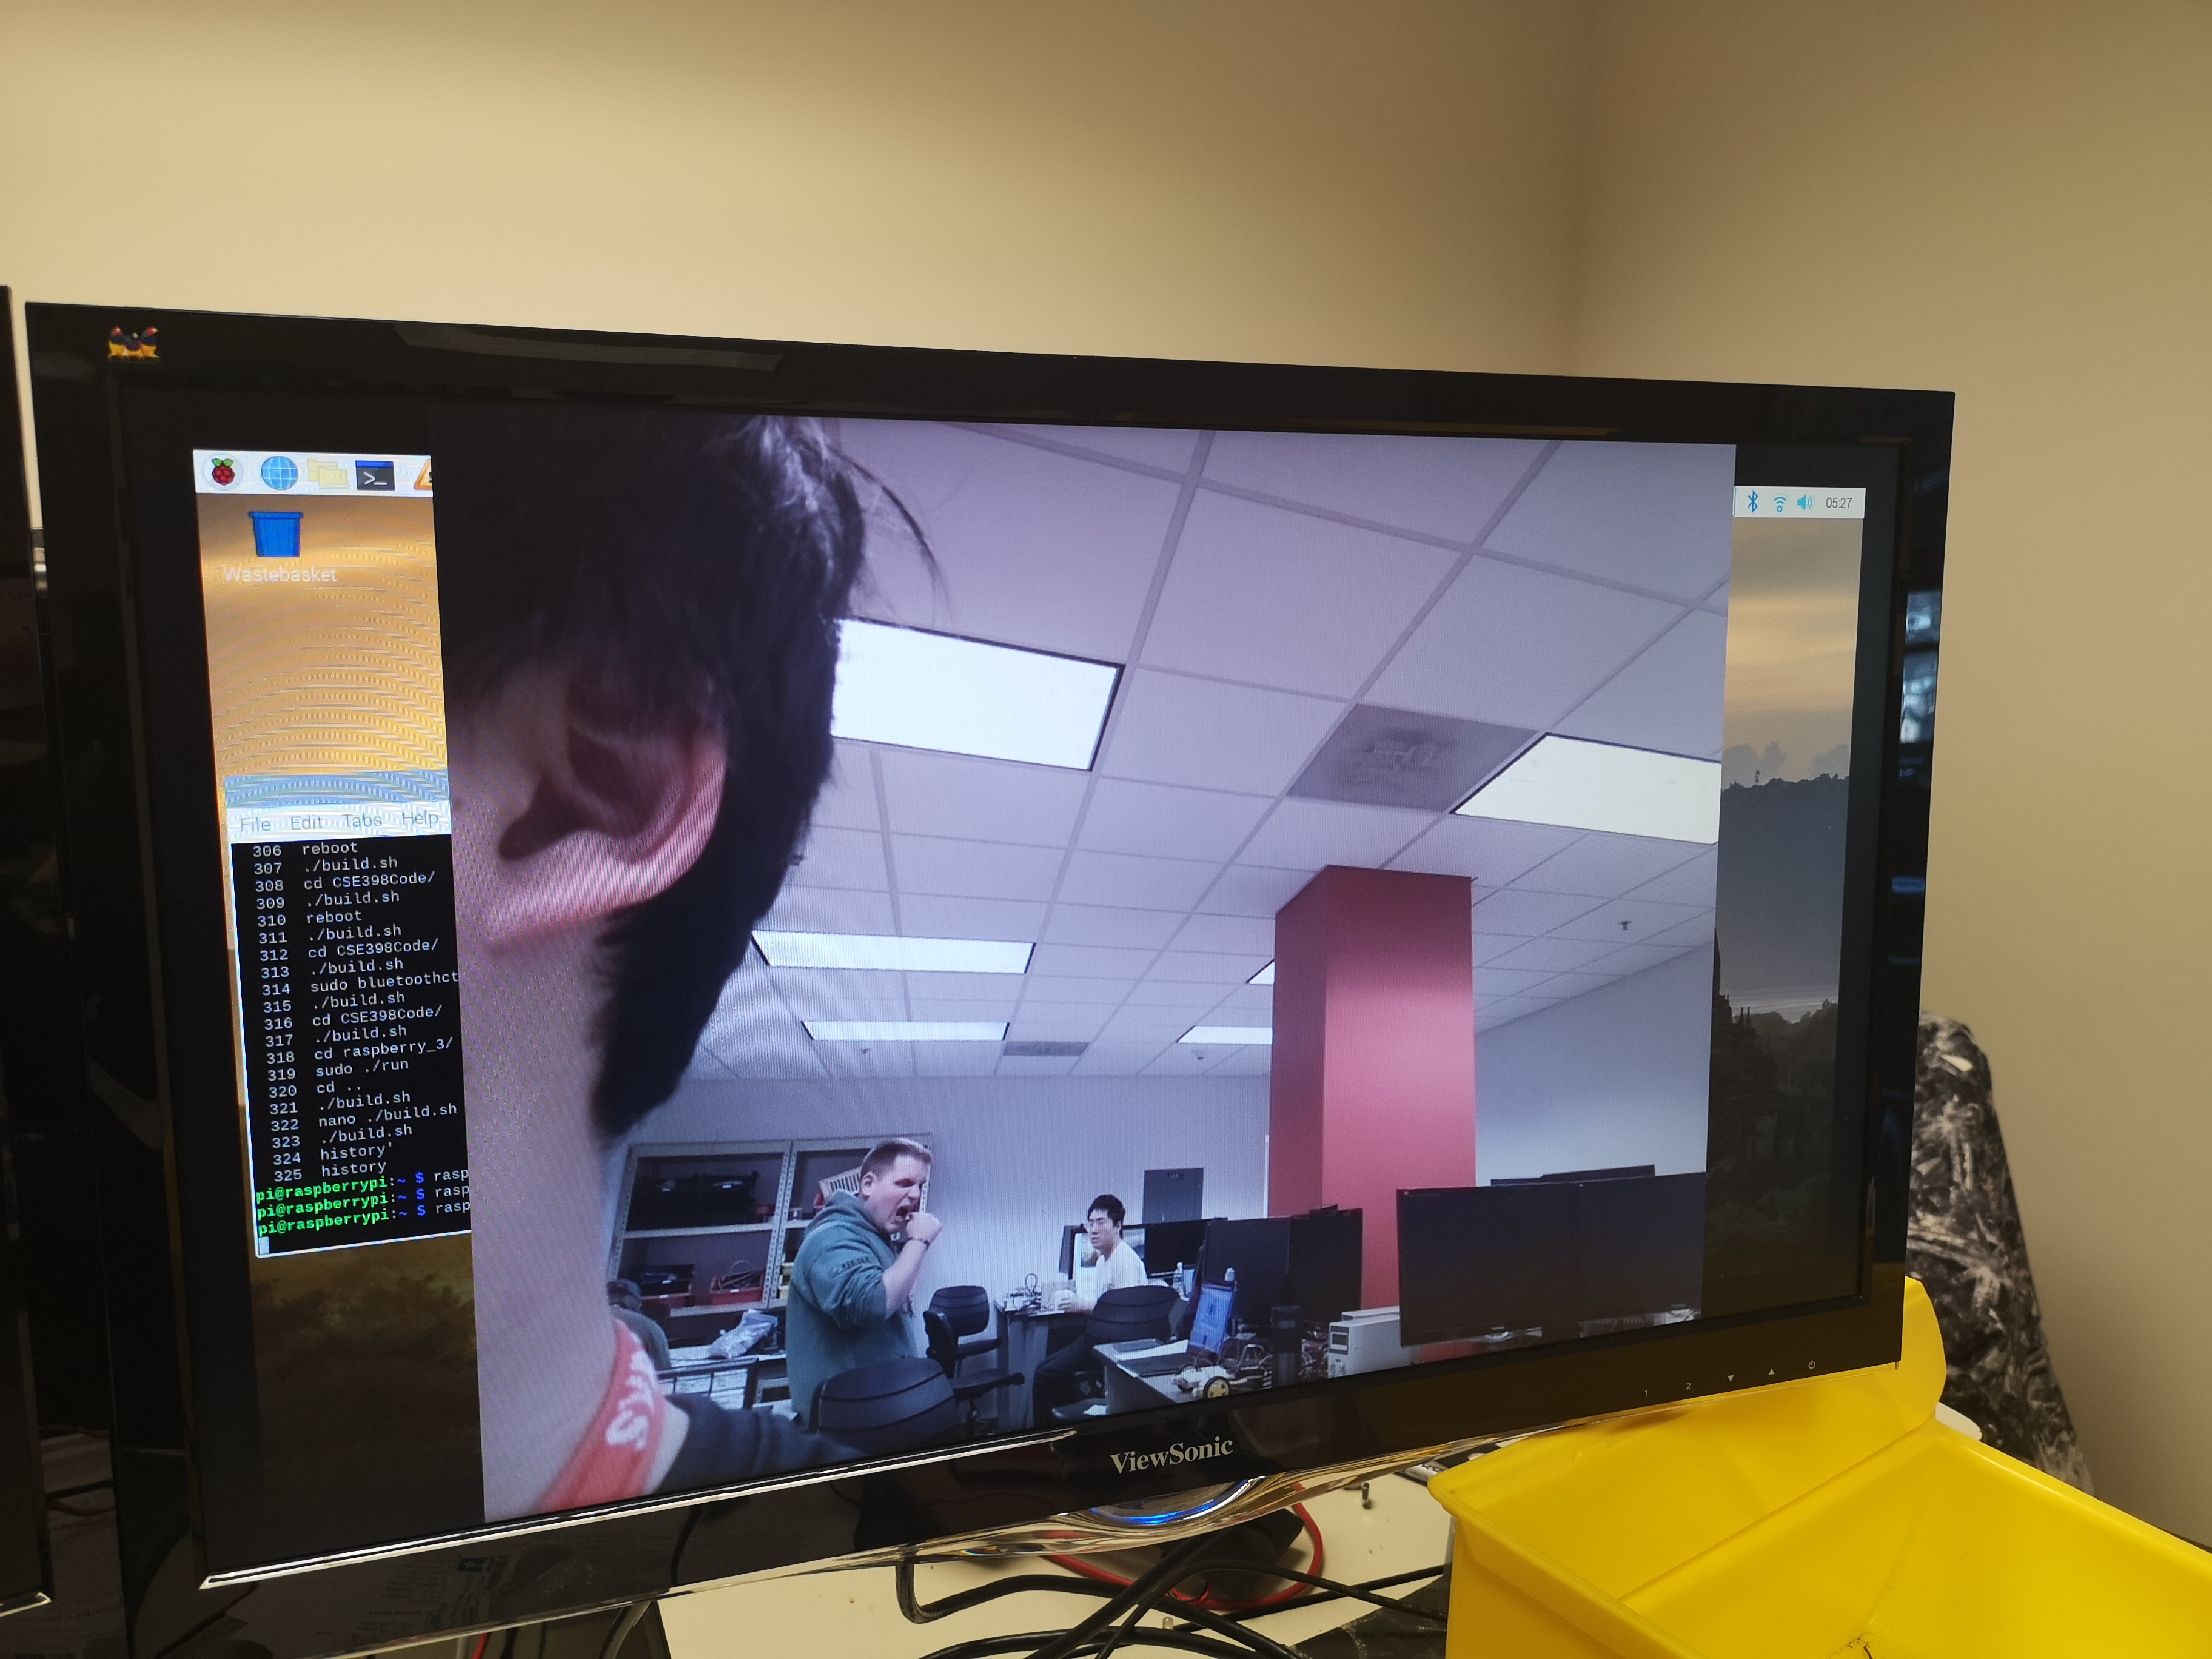
\includegraphics[width=0.5\textwidth]{img/Lab03_14.jpg}
	\caption{Picture Take By Raspistill} 
	\label{BBD}
\end{figure}
\clearpage

\section{Install OpenCV, check with -version \& Get image using OpenCV \& Face recognition using OpenCV}
\subsection{Setup}
In order to make the Raspberry Pi to get image and face recognition using OpenCV, following items is require.
\begin{itemize}
	\item Raspberry PI 3B
	\item SD card
	\item Raspberry Camera
\end{itemize}
\subsection{Procedure}
To finish this task take three steps.
\subsubsection{Install OpenCV and create program}
	To install the openCV, run following command \textbf{sudo apt-get install libopencv-dev}.
	\\\\
	The program take three parts.\\
	The first part is to get the video device from the system.\\
		\begin{lstlisting}
	VideoCapture cap;
	// open the default camera,
	 use something different from 0 otherwise;
	// Check VideoCapture documentation.
	if(!cap.open(0))
		return 0;
		\end{lstlisting}
	The second part is to get image frame from the video device.
		\begin{lstlisting}
	Mat frame;
	cap >> frame;
	if( frame.empty() ) 
		continue; // end of video stream
		\end{lstlisting}
	The third part is to put the image to the face recognition and send out the face location.
		\begin{lstlisting}
			FaceLoc f=detectAndDisplay(frame);
		\end{lstlisting}
		Because the speed of the Raspberry Pi, some change in the face recognition program required to improve the perform.\\
		\textbf{face\_cascade.detectMultiScale( frame\_gray, faces, 1.1, 2, 0|CV\_HAAR\_SCALE\_IMAGE, Size(100, 100));}\\
		Decreasing the size of face recognition will improve the speed.
		\begin{lstlisting}
	FaceLoc detectAndDisplay( Mat frame ){
		std::vector<Rect> faces;
		Mat frame_gray;
		int frame_y= frame.rows;
		int frame_x= frame.cols;
		// cout <<endl; 
		cvtColor( frame, frame_gray, CV_BGR2GRAY );
		equalizeHist( frame_gray, frame_gray );
			
		//-- Detect faces
		face_cascade.detectMultiScale( frame_gray, faces, 1.1, 2,
		 0|CV_HAAR_SCALE_IMAGE, Size(100, 100) );
		Point center( frame_x*0.5, frame_y*0.5 );
		ellipse( frame, center, Size( 20, 20), 0, 0, 360, 
		Scalar( 255, 0, 255 ), 4, 8, 0 );
		FaceLoc f;
		f.x=0;
		f.y=0;
		for( size_t i = 0; i < faces.size(); i++ )
		{
			Point center( faces[i].x + faces[i].width*0.5,
			 faces[i].y + faces[i].height*0.5 );
			ellipse( frame, center, Size( faces[i].width*0.5,
			 faces[i].height*0.5), 0, 0,
			  360, Scalar( 255, 0, 255 ), 4, 8, 0 );
			f.x=faces[0].x+ faces[0].width*0.5-(frame_x*0.5);
			f.y=faces[0].y + faces[0].height*0.5-(frame_y*0.5);
		}
		imshow("this is you, smile! :)", frame);
		waitKey(1);
		return f;
	}
		\end{lstlisting}
\subsubsection{Testing camera}
	The program to test the program is following.
	\begin{lstlisting}
		cap >> frame;
		Mat frame;
		imshow("this is you, smile! :)", frame);
		waitKey(10);
	\end{lstlisting}
	The \textbf{waitKey(10)} is required because the speed of the cpu is too faster. CPU have to wait for the camera to get the image.
\subsubsection{Testing face recognition}
	The program to test the face recognition is following.
	\begin{lstlisting}
		FaceLoc f=detectAndDisplay(frame);
	\end{lstlisting}
	The function for analysis the frame is following.
	\begin{lstlisting}
	FaceLoc detectAndDisplay( Mat frame ){
		std::vector<Rect> faces;
		Mat frame_gray;
		cvtColor( frame, frame_gray, CV_BGR2GRAY );
		equalizeHist( frame_gray, frame_gray );
		
		//-- Detect faces
		face_cascade.detectMultiScale( frame_gray, faces, 1.1, 2,
		0|CV_HAAR_SCALE_IMAGE, Size(100, 100) );
		Point center( frame_x*0.5, frame_y*0.5 );
		ellipse( frame, center, Size( 20, 20), 0, 0, 360, 
		Scalar( 255, 0, 255 ), 4, 8, 0 );
		FaceLoc f;
		f.x=0;
		f.y=0;
		for( size_t i = 0; i < faces.size(); i++ ){
			Point center( faces[i].x + faces[i].width*0.5,
			faces[i].y + faces[i].height*0.5 );
			ellipse( frame, center, Size( faces[i].width*0.5,
			faces[i].height*0.5), 0, 0, 360, 
			Scalar( 255, 0, 255 ), 4, 8, 0 );
		}
		imshow("this is you, smile! :)", frame);
		waitKey(1);
		return f;
	}
	\end{lstlisting}
\subsection{Result}
After use the camera test program, one windows will appear and a video stream will display.
\begin{figure}[hb]
	\centering
	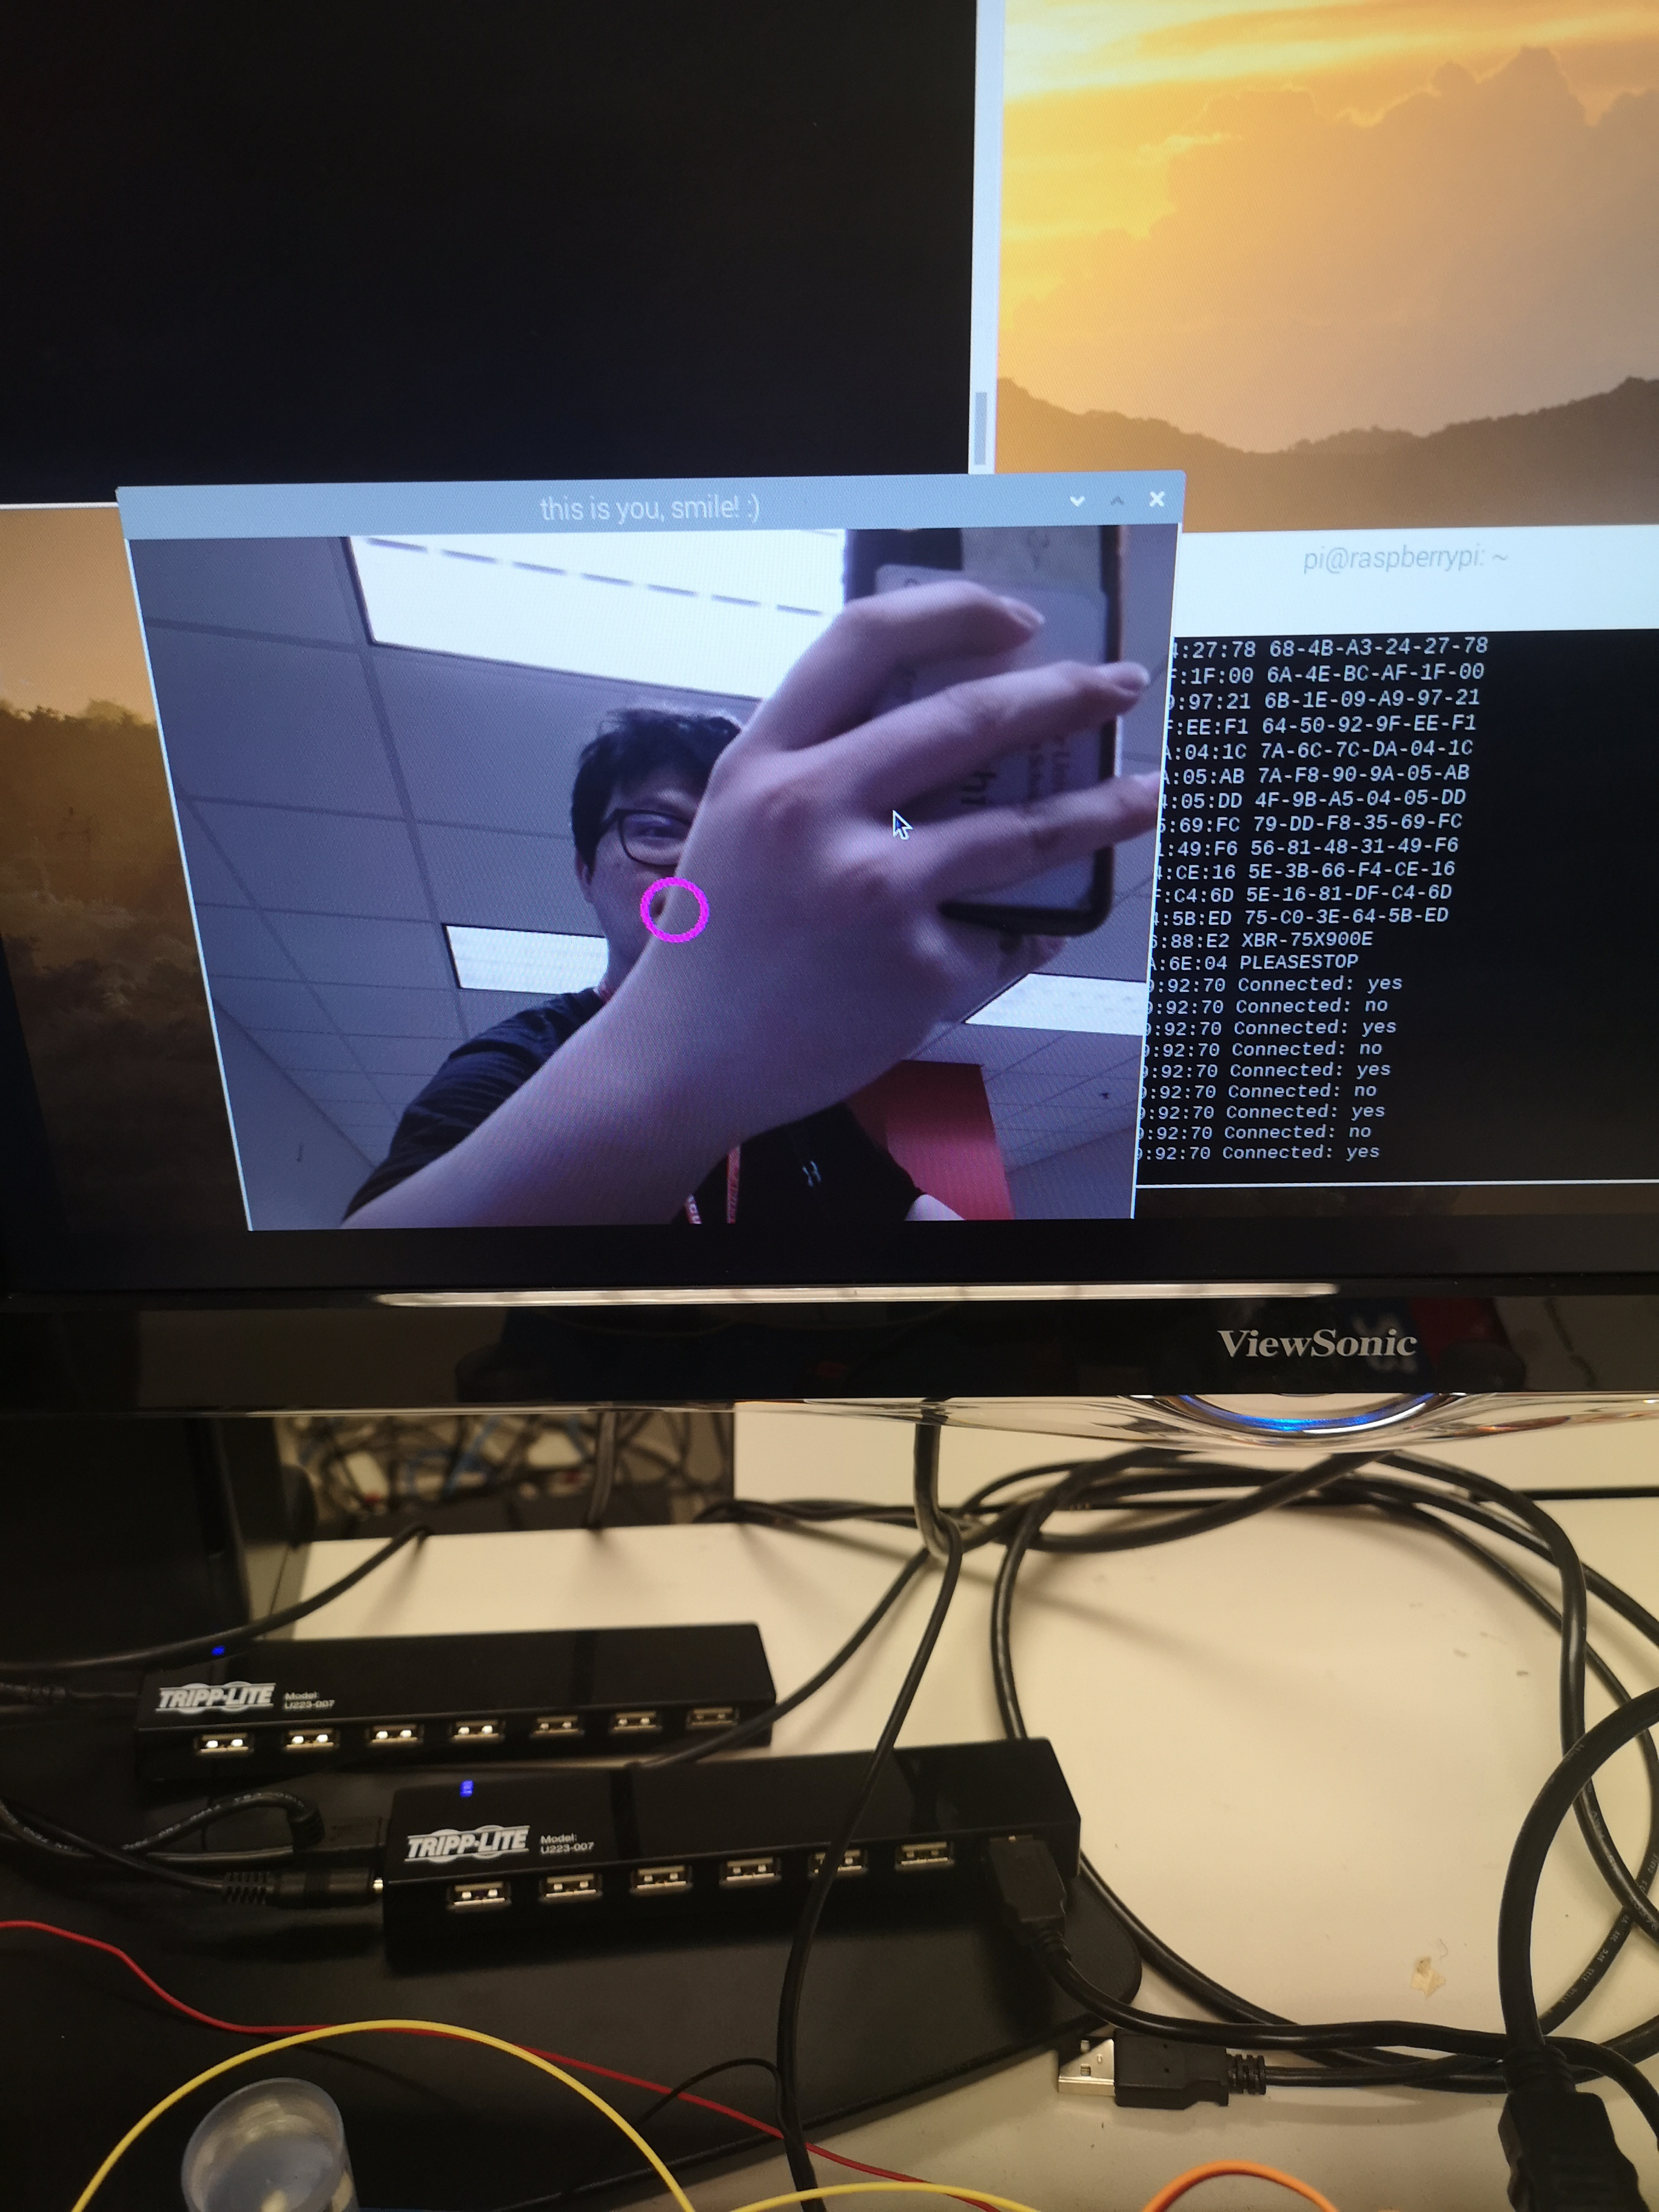
\includegraphics[width=0.5\textwidth]{img/Lab03_11.jpg}
	\caption{Image From OpenCV} 
	\label{BBD}
\end{figure}
After load the face recognition program, the faces in the video will be marked by a red cycle around it.
\begin{figure}[hb]
	\centering
	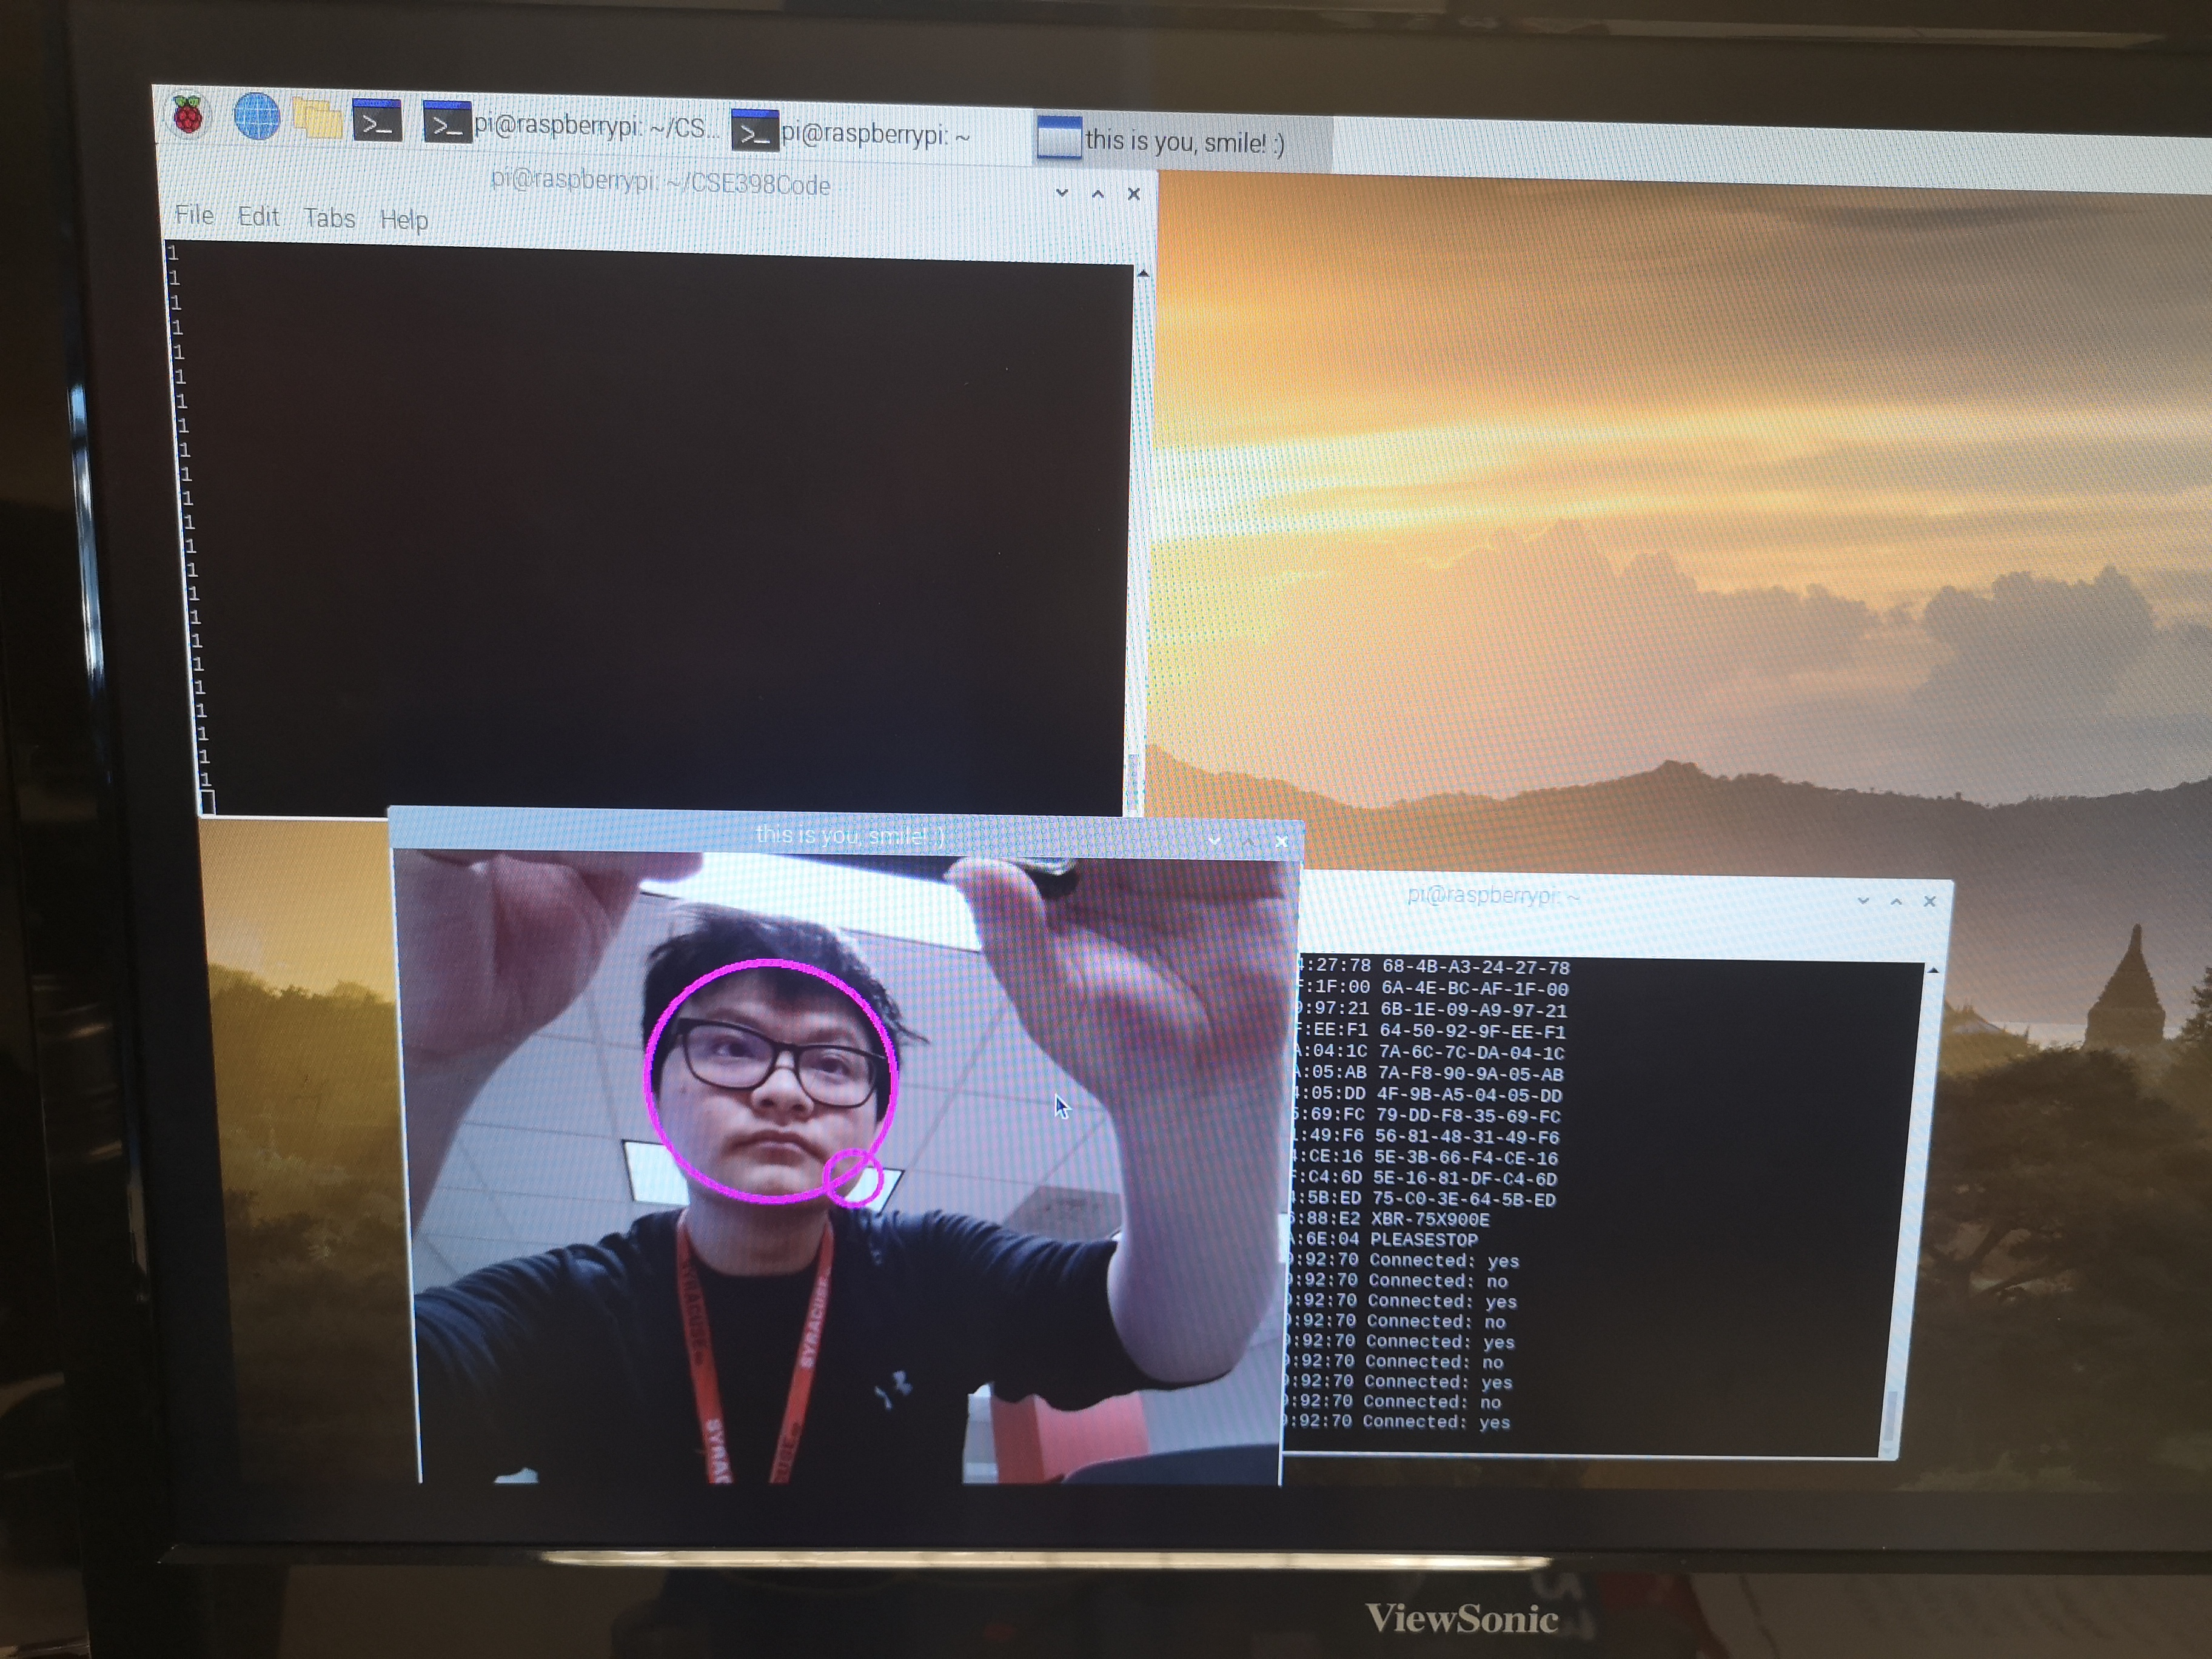
\includegraphics[width=0.5\textwidth]{img/Lab03_09.jpg}
	\caption{Face Recognition With OpenCV} 
	\label{BBD}
\end{figure}
\clearpage
\section{Track Face, keep face centered \& Add BT command: PTU control + Track On/Off}
\subsection{Setup}
In order to make the Raspberry Pi to get image and face recognition using OpenCV, following items is require.
\begin{itemize}
	\item Raspberry PI 3B
	\item SD card
	\item Raspberry Camera
	\item PCA9685
	\item Power Supply
	\item Analog Discovery
	\item PTU
\end{itemize}
\subsection{Procedure}
	To finish this task, the all the program that use in the previous lab is required. The program take three parts.
	\subsubsection{PWM controller}
		The PWM controller is use the \textbf{Adafruit\_PWMServoDriver}. The PTU require two servo. It require two pwm port to operate.  
		\begin{lstlisting}
	pwm.begin();
	pwm.setOscillatorFrequency(27000000);
	pwm.setPWMFreq(SERVO_FREQ);
	
	......
		
	if (f.x>0)h--;
	if (f.x<0)h++;
	if (f.y>0)v++;
	if (f.y<0)v--;
				
	if (h>turn[0])h=turn[0];
	if (h<turn[2])h=turn[2];
	if (v>rise[0])v=rise[0];
	if (v<rise[2])v=rise[0];
				
	pwm.setPWM(0, 0, h);
	pwm.setPWM(1, 0, v);
		\end{lstlisting}
	\subsubsection{Bluetooth controller}
		The bluetooth controller is a little bit different. Because the read is block method, it is impossible to run pwm and listening bluetooth message in the same time. Therefore, multi-thread is required in the program.
		\begin{lstlisting}
void readInput(){
	while (1){
		string goodone=rout.readRF();
		if ((goodone)[0]=='M'){
			cout << "TP3" << endl;
			on=0;
		}
		if ((goodone)[0]=='L'){
			cout << "TP3" << endl;
			on=1;
		}
	}
}
		\end{lstlisting}
		The function above is use to receive the message from the bluetooth that send by phone. It will be running in another thread.
		\begin{center}
		\textbf{thread t(readInput);}
		\end{center}
	\subsubsection{Camera and Face Recognition Handler}
		The camera and face recognition handler is use to in take in the image flow from the camera and run a face recognition process on the frame.
		\begin{lstlisting}
	Mat frame;
	cap >> frame;
	if( frame.empty() ) 
		continue; // end of video stream
	FaceLoc f=detectAndDisplay(frame);
		\end{lstlisting}
		By using the statement above, the image from camera will be send to face recognition process and the location of the face in the frame. Those information will be use to adjust the PTU to make it point to the correct location of the face.
\subsection{Result}
	After load all the program to Raspberry Pi, camera will looking for the face appear in the frame and control the PTU to make the camera point to the center of the face it detected.
	\begin{figure}[hb]
		\centering
		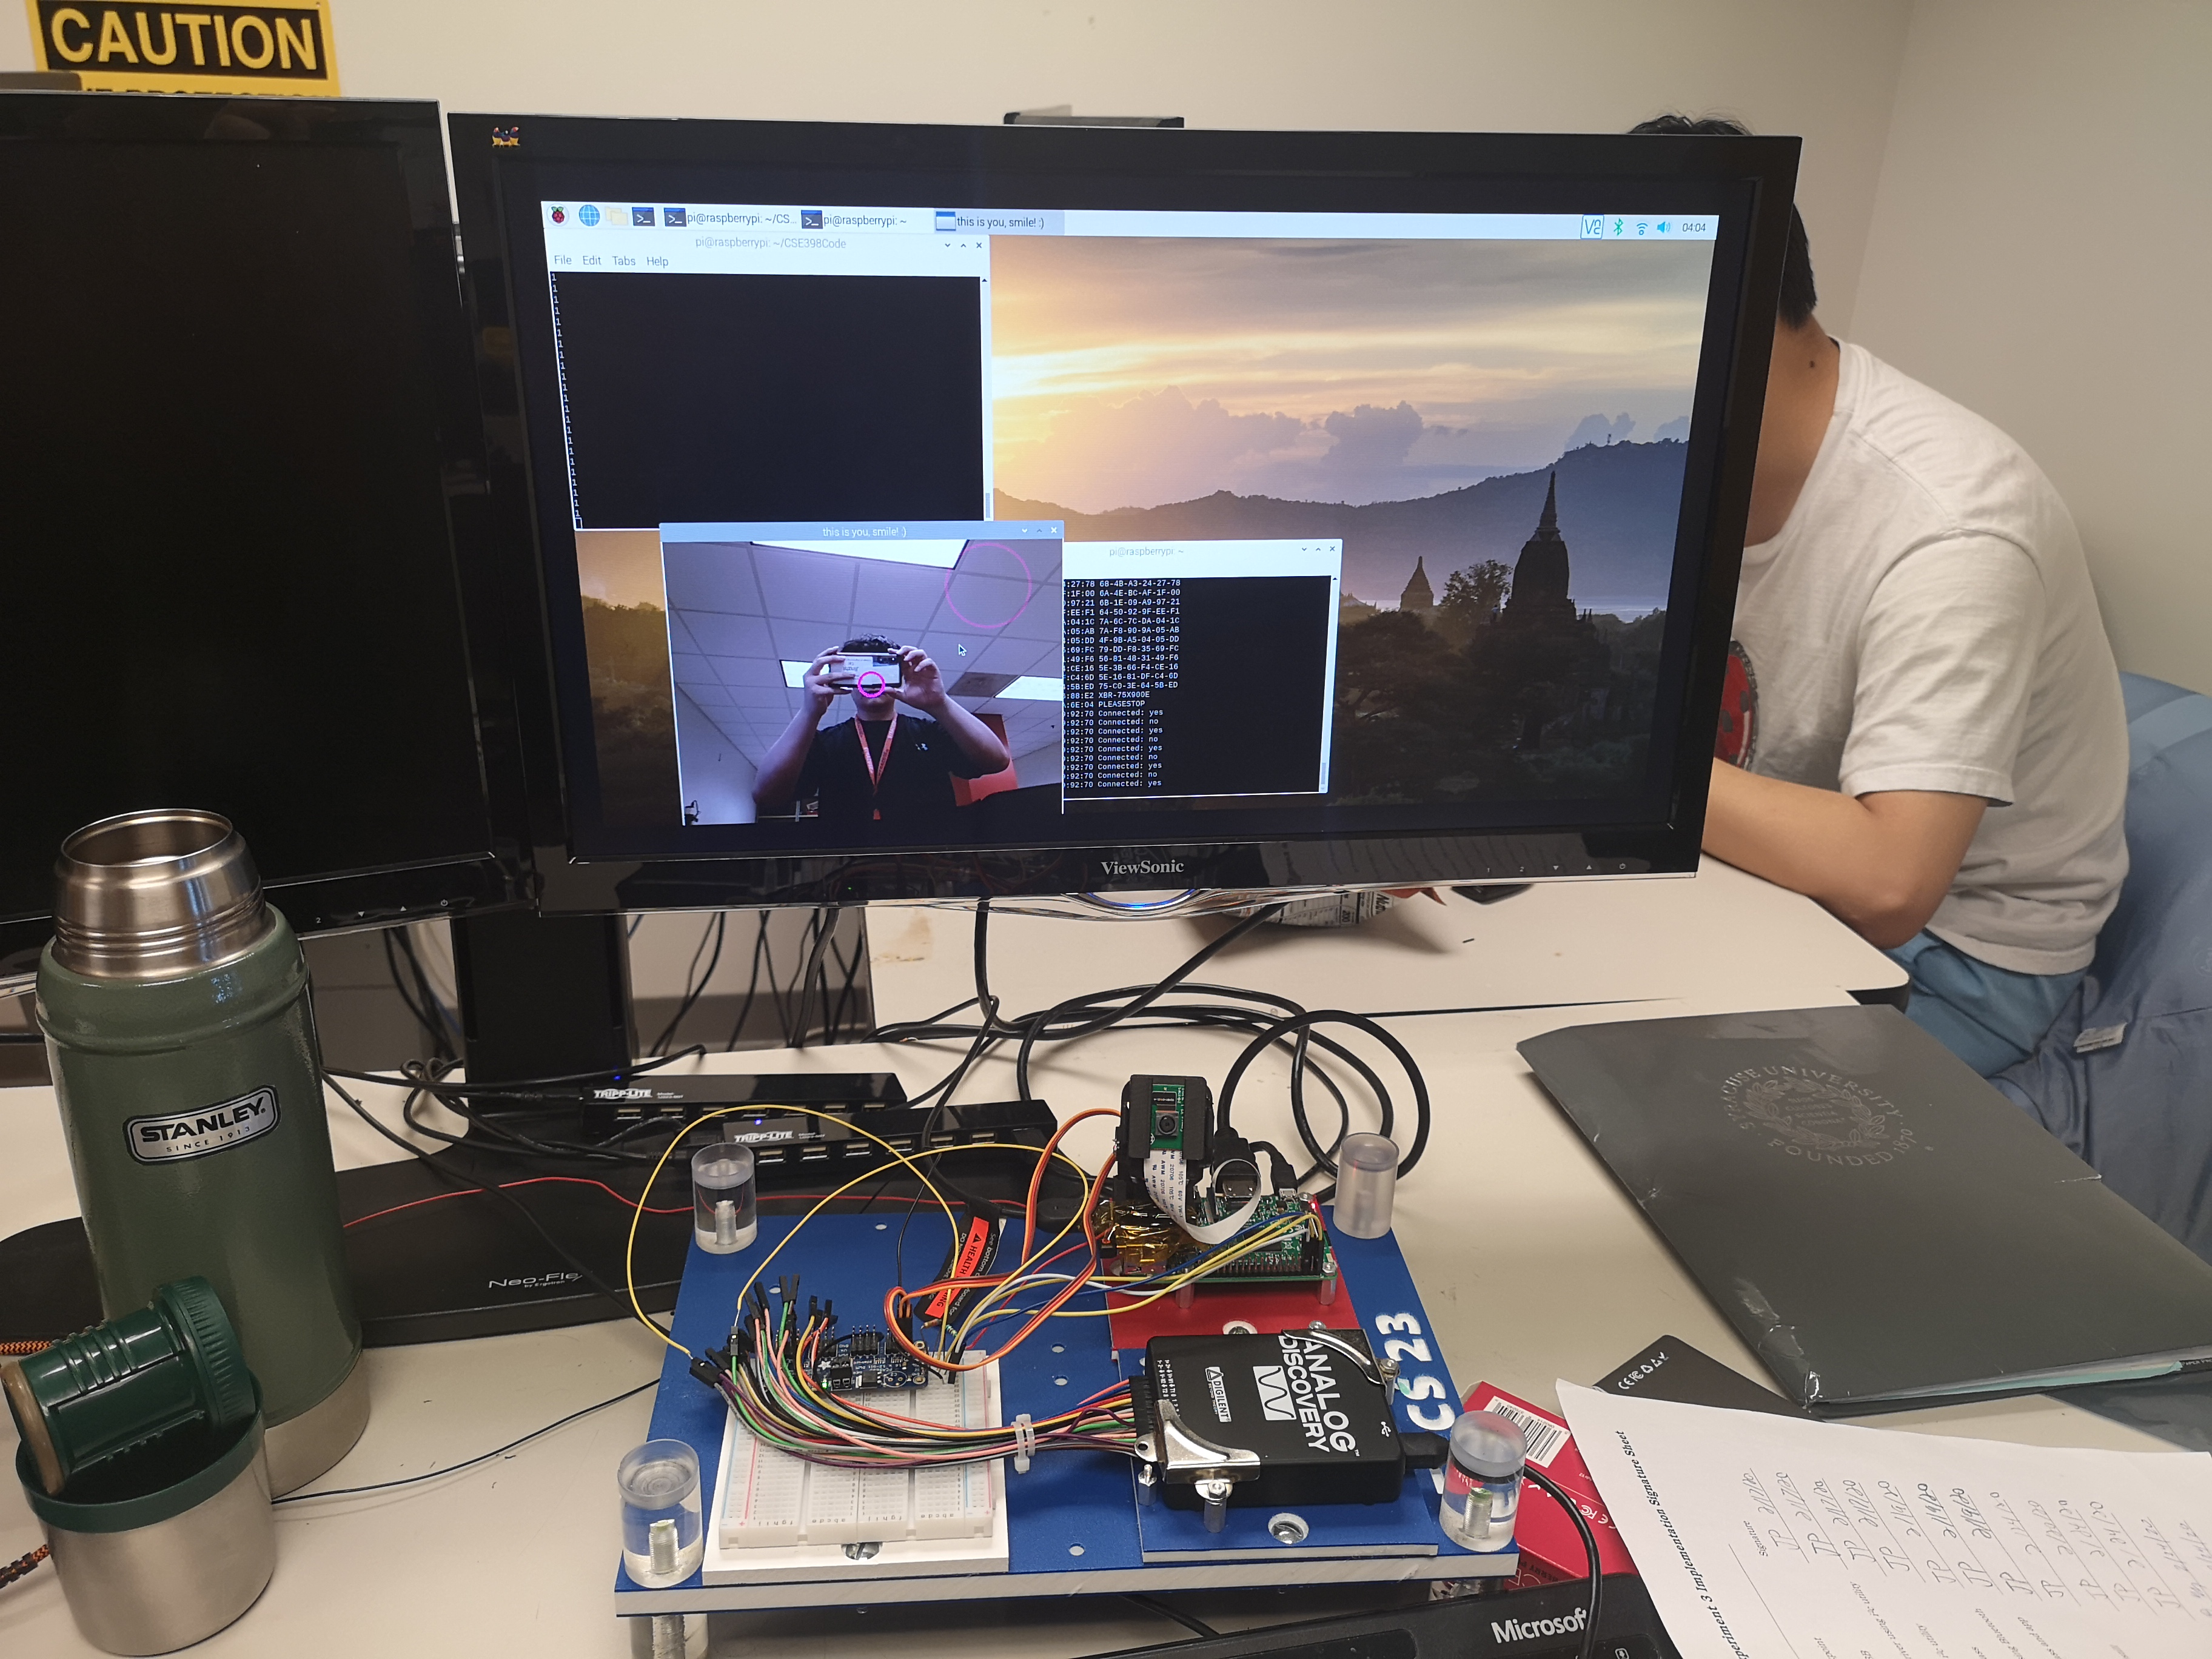
\includegraphics[width=0.5\textwidth]{img/Lab03_08.jpg}
		\caption{Workbranch Setup With Screen} 
		\label{BBD}
	\end{figure}
	\begin{figure}[hb]
		\centering
		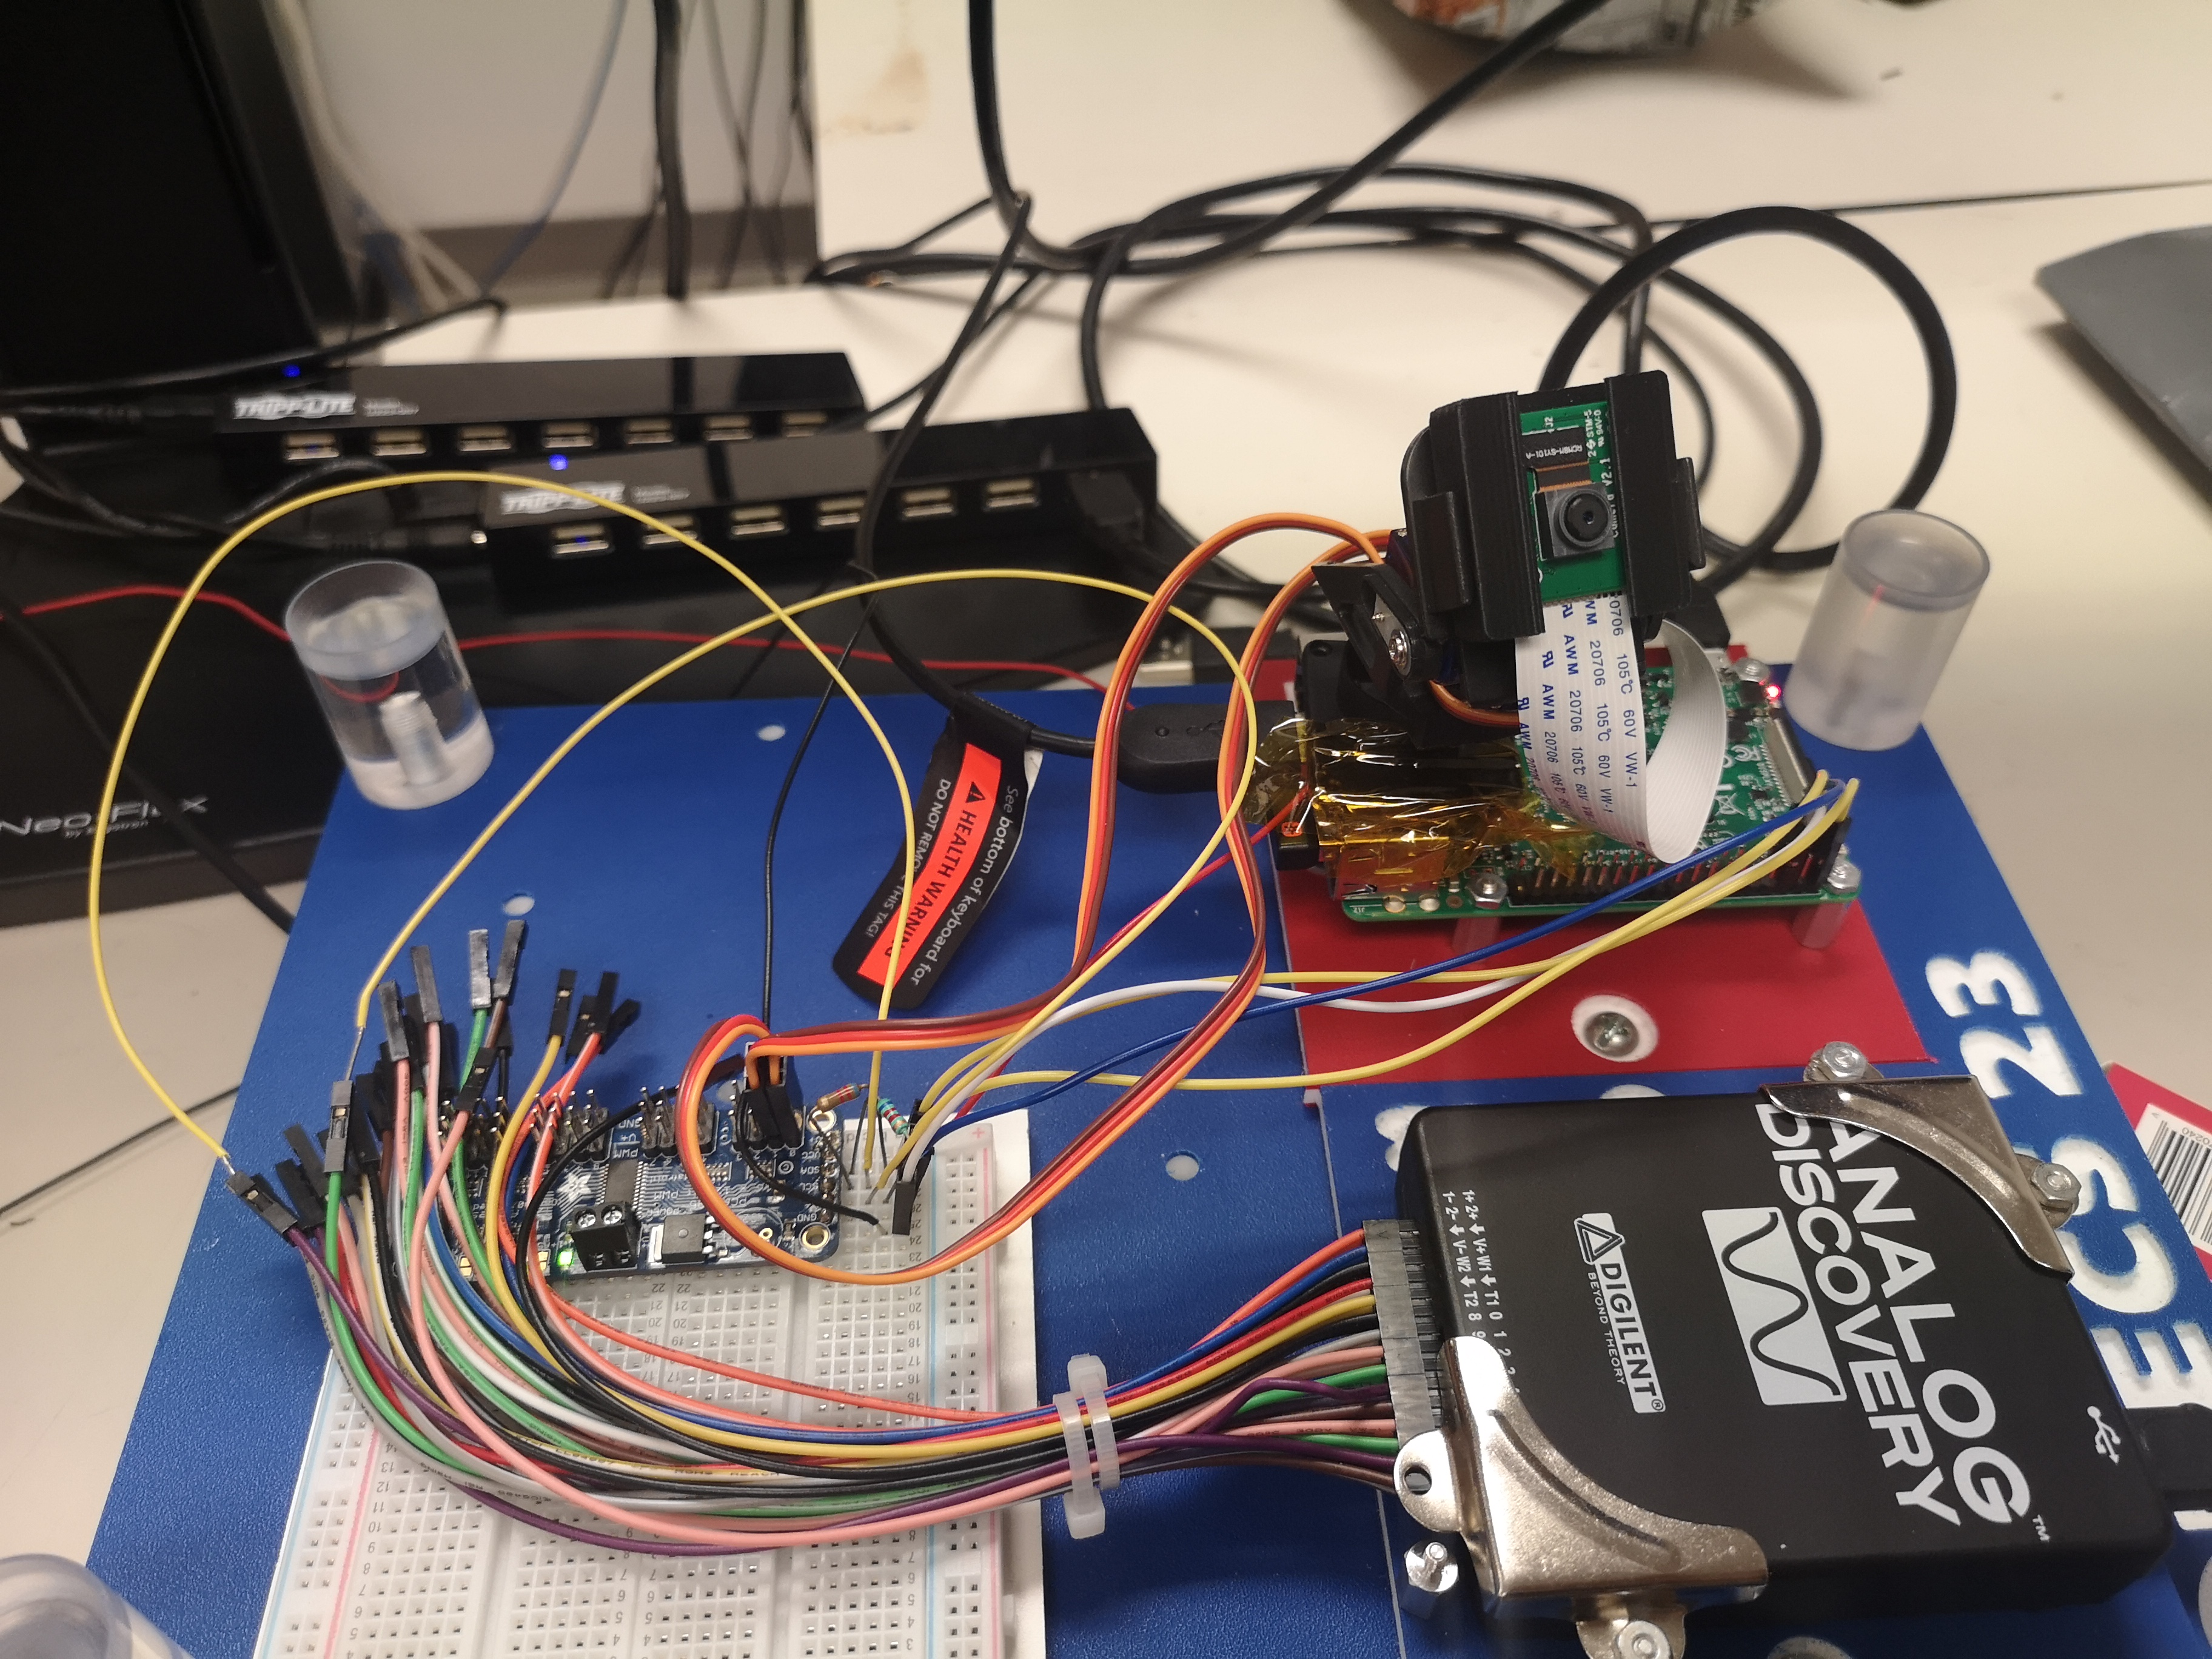
\includegraphics[width=0.5\textwidth]{img/Lab03_13.jpg}
		\caption{Workbranch Setup} 
		\label{BBD}
	\end{figure}
	\begin{figure}[hb]
		\centering
		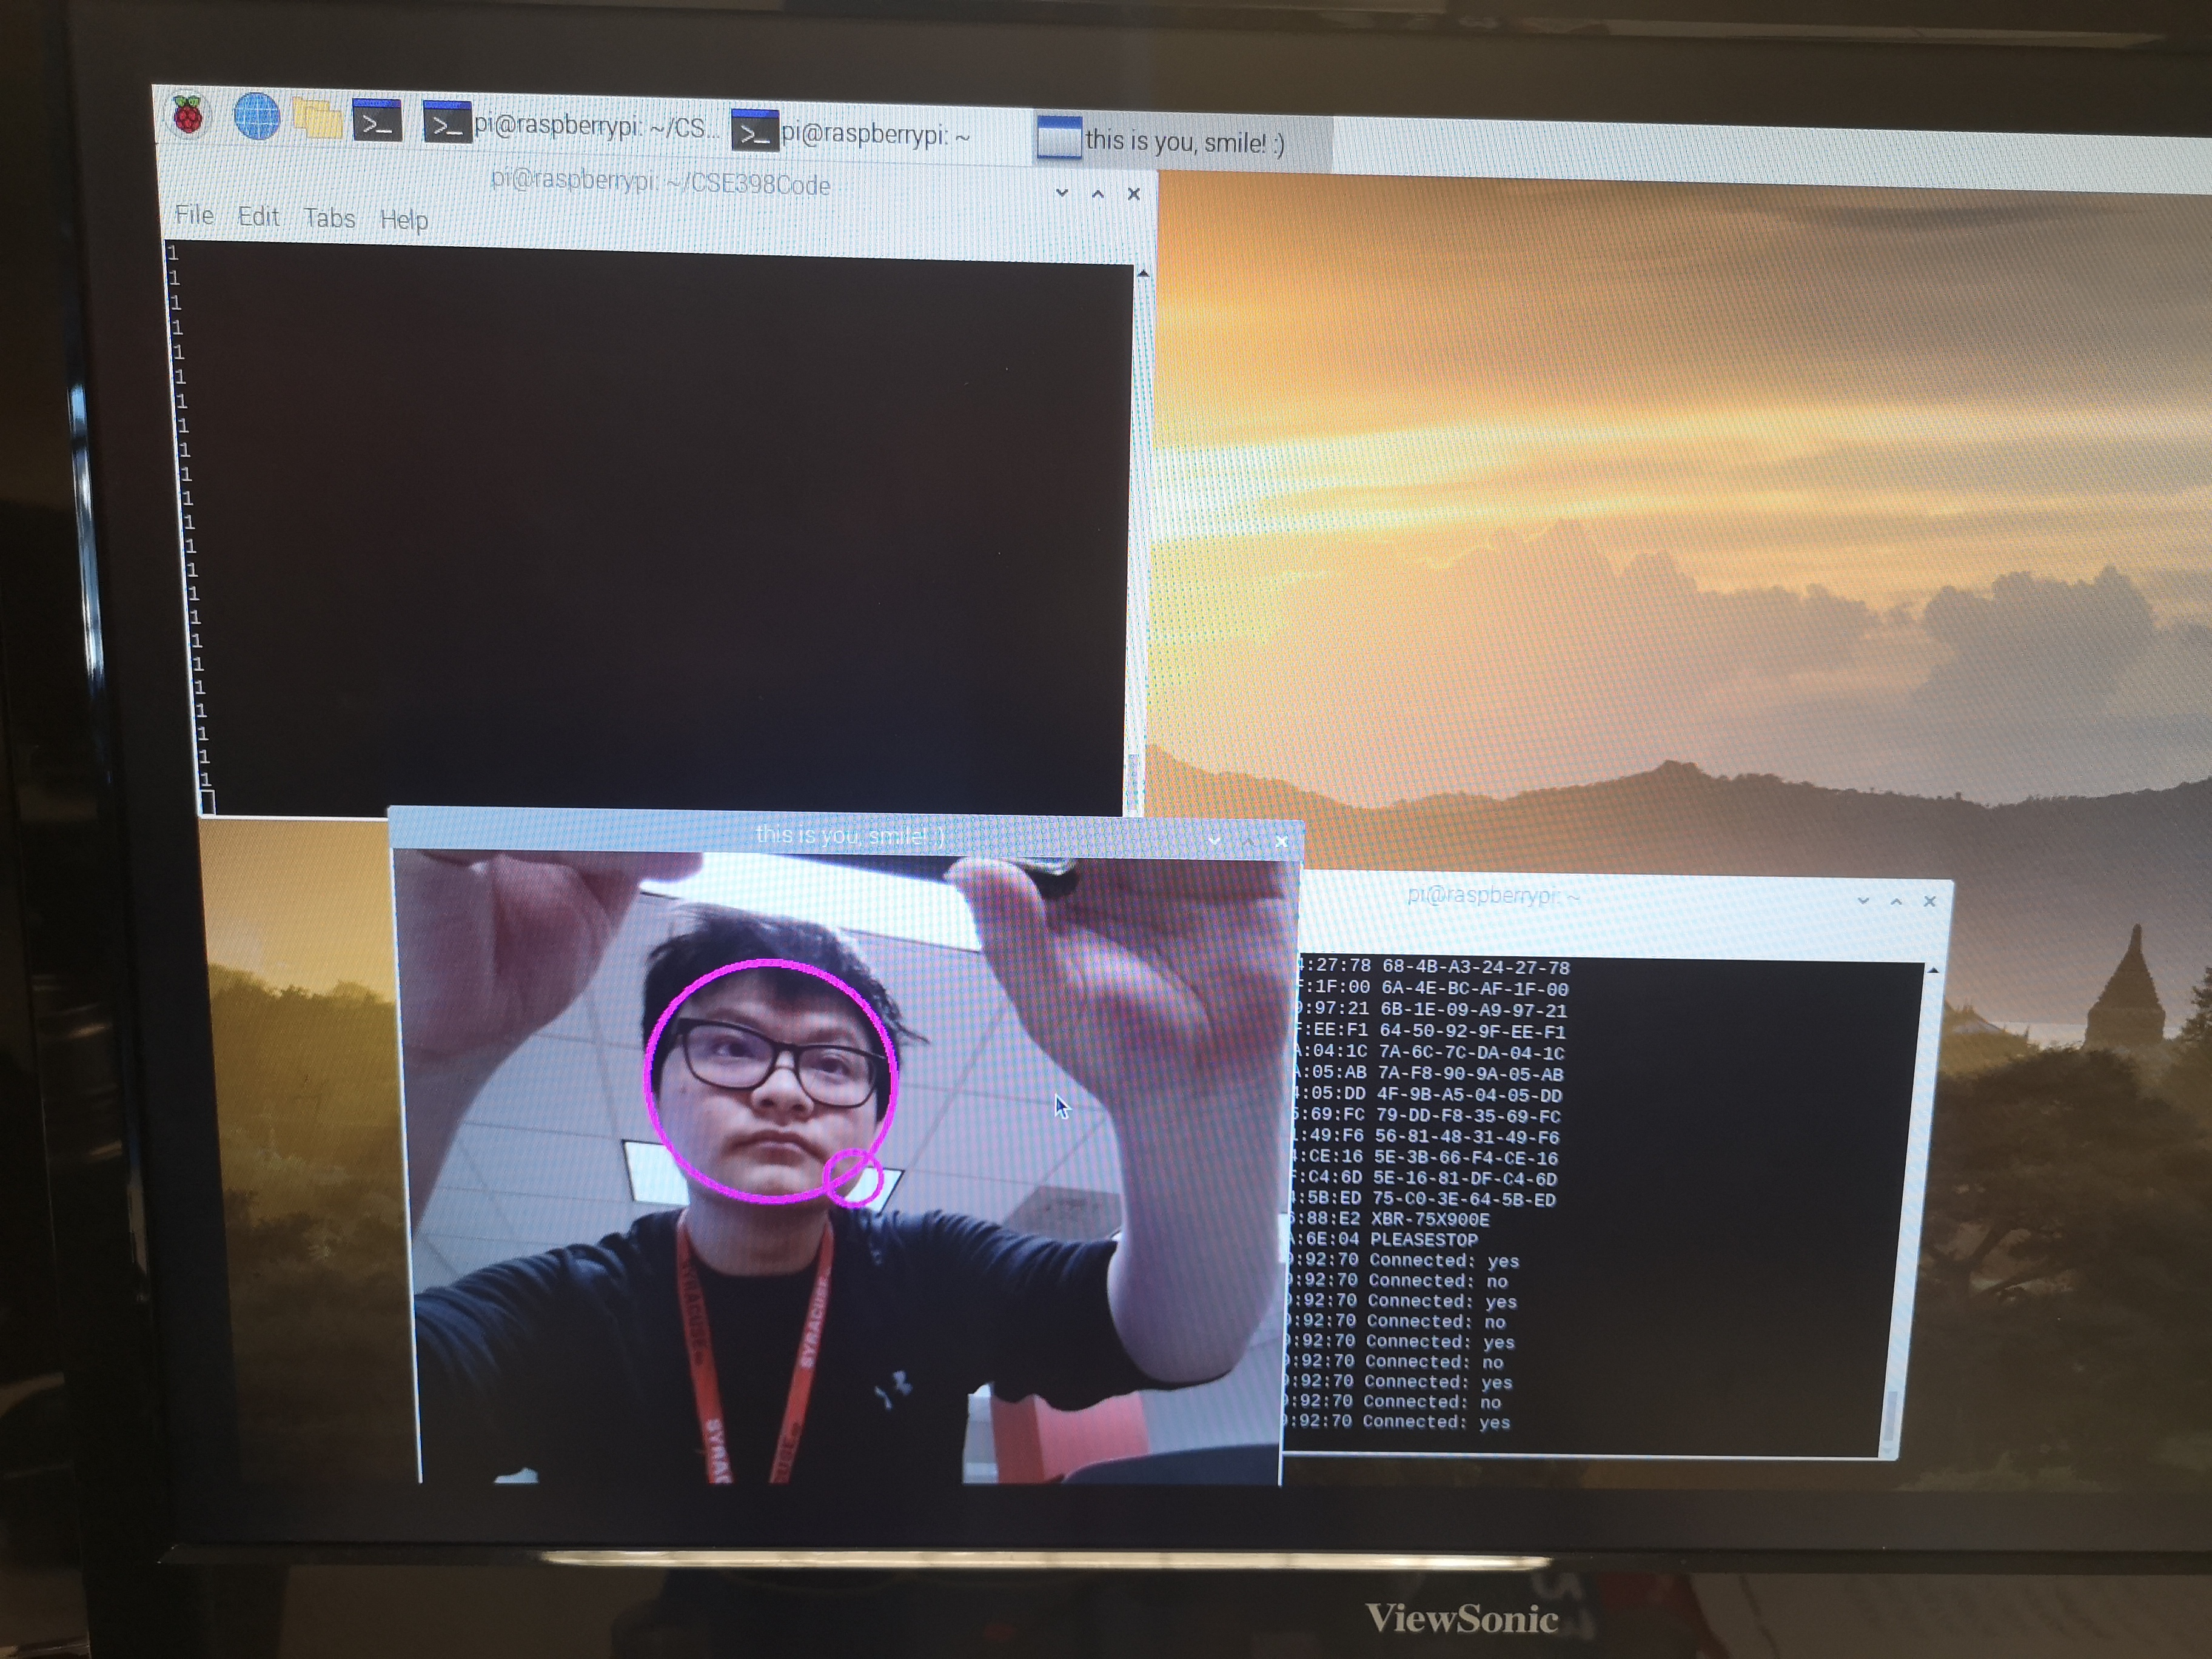
\includegraphics[width=0.5\textwidth]{img/Lab03_09.jpg}
		\caption{Face Recognition With OpenCV} 
		\label{BBD}
	\end{figure}
\clearpage
\section{Conclusion}
The embedded computing system is a very key part in the everyday life. By running this lab, we understand the structure of Raspberry Pi hardware, the way it communicate with the internal system, and how it display in the .  The face tracking system we design, can apply a lot of different place such as surveillance cameras. As the computer system that the most close the physical world, many bug is not only coming from in the software layer but also the hardware connection. It create new challenge to the hardware engineers to fix the systems that have problems. However, it will have greater use also because it close to the physical world people are involved in. 

\end{document}